\chapter{Langevin Equations}\label{ch:langevin}

In Chapter 16, we have discussed how a drunkard walks around using a random walk model, which assumes that the random walker hops from one site to another at random.  That model uses a discrete time, discrete steps, and discrete directions.  However, the real drunkard does not walk in such a way.  It walks in continuous time and space.  The continuous random walk has been a very useful mathematical model in many parts of physics and other fields of science. 

A most popular example is a Brownian motion.
Consider a bead which is much bigger (heavier) than water molecules but small enough to experience individual water molecules.  From the view point of the bead, a liquid water is not a continuous media.  However, individual water molecules are so small that the impulse by a single collision is not big enough to change the motion of the bead.  Many collisions over a certain period of time are necessary. (See Fig. \ref{fig:brownian_particle})  On the other hand, the collisions happen in all directions and on average the net impulses tend to cancel out.  However, the net impulse is not exactly zero and fluctuates due to the finite number of collisions.  Occasionally bigger impulse from the left than from the right and then the net force to the right is exerted on the Brownian particle. Therefore, the bead is subject to a random force. In other words, the force on the bead is a stochastic variable. Einstein is the first person to explain the Brownian motion using a mathematical model based on the probability distribution of the particles in the surrounding liquid.\cite{brownian_movement_einstein}  Another approach based on the trajectory of the Brownian particle was developed by Langevin at a later time.\cite{langevin_eq_lemons}  The equation of motion for the Brownian particle is known as the Langevin equation.\cite{langevin_eq_zwanzig,langevin_eq_sekimoto}  It is a kind of differential equations but contains random forces and thus the solution is also stochastic.  Even when the initial condition is uniquely specified, realized trajectories never be the same. We call such differential equation stochastic differential equation (SDE) in contrast to ODE.  The numerical methods to solve SDE is similar to those for ODE but the random force must be treated in a different way from the regular forces.


\begin{figure}
\centering
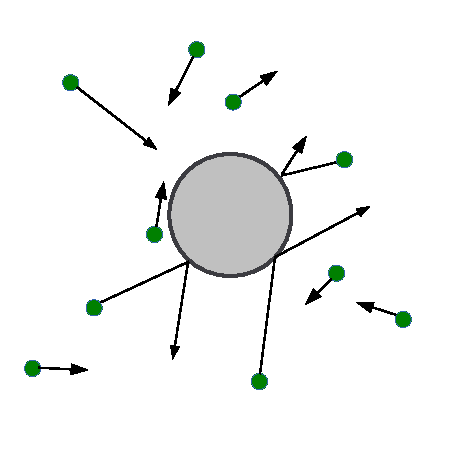
\includegraphics[width=2in]{18.Langevin/brownian_particle.pdf}
\caption{A heavy particle experiences many collisions with smaller particles but its velocity remains the same for a certain short period of time.   The force exerted on the particle is the sum of the forces by individual collisions over a period of time.  In most times, the net force is nearly zero because collisions take place on every direction.  However, the number of collisions is finite and fluctuates from time to time. Therefore, the net force also fluctuates and occasionally it is big enough to change the velocity of the particle appreciatively.}
\label{fig:brownian_particle}
\end{figure}

\section{Langevin equation}

\subsection{Definition}
Microscopically, the motion of the bead and water molecules are determined by a set of Newton's equations of motion.  However, the number of equations is too great to solve analytically.  Since we are interested in the motion of the bead, we want to find an effective equation of motion without the detailed knowledge of the trajectories of water molecules.  Langevin developed such an equation. It is a Newton's equation for the bead but with a random force due to the collision with the water molecules. A typical form of the Langevin equation is
\begin{equation}\label{eq:langevin}
M \ddot{X} = -\gamma \dot{X} +  \alpha \xi(t) + F_\text{ext}(X,t)
\end{equation}
where $M$ and $X$ are the mass and the position of the Brownian particle.  $F_\text{ext}$ is deterministic external force such as gravity. The effect of collisions with the water molecules appears in two parts.  One is the drag force $-\gamma \dot{X}$ where $\gamma$ is the frictional coefficient. The drag office is due to the fact that when the Brownian particle is moving more collisions take place in one direction than other direction.  The other is a random force $\alpha \xi(t)$ where $\alpha$ is a constant to be determined.  As we discussed above, the average of the random force is zero.  In addition, the random force at time $t$ is independent of the random force at a different time $t'$.  Putting theses condition in mathematical form, we define the properties of the stochastic function $\xi(t)$ by
\begin{equation}\label{eq:GW_noise}
\mean{\xi(t)}=0, \qquad \mean{\xi(t) \xi(t')} = \delta(t-t')
\end{equation}
where $\delta(\cdot)$ is the delta function.  Furthermore, we learned in Chapter 16 that the sum of many random numbers is Gaussian distributed.  
Therefore, the random force, which is the sum of many random collisions, is also Gaussian distributed.  Then, the Gaussian stochastic variable is uniquely determined by the mean and variance (\ref{eq:GW_noise}).  This type of stochastic variable is commonly called Gaussian white noise.\footnote{The power spectrum of the random force does not depend on the frequency and thus includes all frequencies with equal strength.  The situation is similar to \textit{white} color which consists of all colors (frequencies).}

Now we will determine the value of $\alpha$.
When there is no external force, the Brownian particle reaches a thermodynamic equilibrium after sufficiently long time and the equipartition theorem\cite{equipartition} suggests that  $\displaystyle\frac{M}{2}\mean{\dot{X}^2} \xrightarrow{t \rightarrow \infty} \displaystyle\frac{\kB T}{2}$.  This condition uniquely determines the strength of the random force.
Using the Langevin equarion (\ref{eq:langevin}) and the definition of Gaussian noise  Eq. (\ref{eq:GW_noise}),  the mean square velocity is give by
\begin{equation}
\mean{\dot{X}^2} = \me^{-2 \gamma t/M} \dot{X}(0)^2 + \frac{\alpha^2}{2\gamma M} \left ( 1- \me^{-2\gamma t/M} \right )
\xrightarrow{t \rightarrow \infty} \frac{\alpha^2}{2\gamma M}.
\end{equation}
With the help of the equipartition theorem, we obtain
\begin{equation}
\alpha = \sqrt{2 \gamma \kB T}.
\end{equation}
See Ref. \cite{langevin_eq_zwanzig} for detailed derivation.

The mean square displacement can be also  analytically computed using Eq. (\ref{eq:GW_noise})
and the result is
\begin{equation}\label{eq:msd_full}
\mean{(X(t)-X(0))^2} = \left( \frac{\alpha}{\gamma}\right)^2 \left [ t - \frac{M}{\gamma} \left (1- \me^{-\gamma t/M} \right ) \right ]
\xrightarrow{t \gg M/\gamma} \frac{2\kB T t}{\gamma}
\end{equation}
from which we find the diffusion constant
\begin{equation}
D = \frac{\kB T}{\gamma}
\end{equation}
This is the famous Einstein relation and an example of the fluctuation-dissipation theorem.\cite{fd_theorem}  Using this diffusion constant, the strength of the random force is expressed as
\begin{equation}
\alpha = \gamma \sqrt{2D}.
\end{equation}

The Stokes frictional coefficient of a spherical particle is given by
\begin{equation}
\gamma = 6 \pi \eta R
\end{equation}
where $\eta$ is the viscosity of the surrounding fluid and $R$ the radius of the Brownian particle.  In general 
the frictional constant depends the mass and density of water molecules, temperature and the shape of the Brownian particle.  To determine it from the experimental observation, one can measure the autocorrelation function of the velocity\cite{langevin_eq_zwanzig}
\begin{equation}\label{eq:autocorr_v}
\frac{\mean{V(\tau)V(0)}}{\mean{V(0)^2}} = \me^{-\gamma t/M} .
\end{equation}
Plotting it in the semi-log scale, the slope is $-\gamma/M$.

\subsection{Overdamped Langevin equations and Wiener Processes}

When the friction is very large, the effect of inertial mass $M$ becomes negligible.  Then, Eq. (\ref{eq:langevin}) can be approximated by
\begin{equation}\label{eq:overdamped}
\dot{X} = \sqrt{2D} \xi(t) + \frac{1}{\gamma} F_\text{ext}(X,t)
\end{equation}
which is known as the overdamped Langevin equation\cite{langevin_eq_sekimoto} and commonly used in biological systems.  For example the motion of a protein  in a cytosol is investigated with the overdampled Langevin equation. 

When $F_\text{ext}=0$, the trajectory $X(t)$ determined by Eq. (\ref{eq:overdamped}) is called the Wiener process which is solely determined by the random force as
\begin{equation}\label{eq:od_displacement}
X(t) = X(0) + \sqrt{2D} \int_0^t \xi(s)\, \md s
\end{equation}
The mean square displacement grows as
\begin{equation}\label{eq:msd_od}
\mean{(X(t)-X(0))^2} = 2D t
\end{equation}
which agrees with Eq. (\ref{eq:msd_full}).


\subsection{Ornstein-Uhlenbeck process}

In the absence of the external force, the Langevin equation (\ref{eq:langevin}) does not depend on the position and is a first order SDE of the velocity
\begin{equation}\label{eq:ou_v}
\dot{V} = -\frac{\gamma}{M} V + \frac{\gamma}{M} \sqrt{2D} \xi(t)
\end{equation}
The solution to this SDE is known as the Ornstein-Uhlenbeck process.

Another example of the  Ornstein-Uhlenbeck process is an overdamped Brownian particle in a harmonic potential. The overdumped Langevin equation fo this particle is given by the  Ornstein-Uhlenbeck process
\begin{equation}\label{eq:ou_x}
\dot{X} = -\frac{k}{\gamma} X + \sqrt{2D} \xi(t)
\end{equation}
where $k$ is the spring constant.  Apart from the parameters, Eq (\ref{eq:ou_x}) is mathematically equivalent to Eq. (\ref{eq:ou_v}).
Assuming that  the Brownian particle is initially located at $X(0)=0$, the mean square displacement is given by
\begin{equation}
\mean{X(t)^2} = \frac{\kB T}{k} \left [ 1 - \me^{-2k t/\gamma} \right ] \xrightarrow{t \rightarrow \infty} \frac{\kB T}{k}
\end{equation}
Hence the mean potential energy satisfies the equipartition theorem\cite{equipartition}
\begin{equation}
\mean{U} = \frac{k}{2}\mean{ X^2} = \frac{\kB T}{2}
\end{equation}
indicating that the Brownian particle asymptotically reaches the thermal equilibrium.

\subsection{Numerical Algorithm: the Heun method}

In order to develop a numerical method for the Langevin equations, we need to understand the Wiener process, in particular the integral of the random force in the overdamped Langevin equation (\ref{eq:od_displacement}) in the absence of the external force.  The stochastic function $\xi(t)$ is not an ordinary function of time and we must be very careful about it.\footnote{The function $\xi(t)$ is continous but not differentiable at any point!}  If $\xi(t)$ were an ordinary function, the integral over infinitesimal time $\md t$ would be proportional to $\md t$:
\begin{equation}
\int_0^{\md t} \xi(s)\md s = g \md t
\end{equation}
where $g$ is a stochastic constant.
Then, the mean square displacement would be
\begin{equation}
\mean{(X(\md t)-X(0))^2} = 2D \mean{g^2} (\md t)^2
\end{equation}
which contradicts with Eq. (\ref{eq:msd_od}).  In order to get the correct relations (\ref{eq:GW_noise}) and (\ref{eq:msd_od}), we conclude that
\begin{equation}\label{eq:wiener}
\int_0^{\md t} \xi(s)\md s = g \sqrt{\md t}.
\end{equation}
with $\mean{g}=0$ and $\mean{g^2}=1$.  Since $\xi$ is Gaussian distributed, $g$ is also Gaissian-distributed.
See Refs \cite{langevin_eq_zwanzig,langevin_eq_sekimoto} for more detailed discussion of the Wiener process.

Now we find a simplest numerical method for the overdamped Langevin equation (\ref{eq:od_displacement}) including the external force.  We assume that the diffusion constant does not depend on $X$ nor $t$.  Integrating Eq. (\ref{eq:overdamped}) from $t$ to $t+h$, 
\begin{equation}
X(t+h)-X(t) = \sqrt{2Dh} g  + \frac{1}{\gamma} \int_t^{t+h} F(X(t'), t') \md t'
\approx  \sqrt{2Dh} g + \frac{1}{\gamma}  F(X(t), t) h
\end{equation}
where we used the Euler method for the integral of the external force.  The value of $g$ is normally a distributed random number. Note that the integral of the random force is exact since $D$ is just a constant.
If the diffusion constant depends on the position, the mathematics of stochastic differential equation is more complicated \cite{langevin_eq_sekimoto} and we do not discuss it here.  The discretization error arises from the Euler method for the external force. As we discussed in Chapter 4, the Euler method is accurate only up to the order of $h$.  A better method is to use the Runge-Kutta or predictor-corrector method for the external force.  The following algorithm, known as the Heun method, is equivalent to the predictor-corrector method (Section 4.2.3) for ODE and accurate up to the order of $h^2$.

\begin{myalgobox}
\Algorithm{Heun method for the overdamped Langevin equation}\label{al:heun_od}

\medskip
\begin{minipage}{5in}
\small
\begin{enumerate}
\item Assuming that $X(t_i)$ is known, we predict $X(t_{i+1})$ where $t_{i+1}=t_i+h$.
\item Generate a normally-distributed random number $g$  (use a Box-Muller method. See Chapter 14.)
\item Generate a random force $G = \sqrt{2D}\, g$.
\item Generate a deterministic force if any
\begin{equation}
F_1 = F_\text{ext}(X(t_i),t_i)/\gamma.
\end{equation}
\item Predict the next $X$ (This is just a first prediction.)
\begin{equation}
X'(t_{i+1}) = X(t_i) + F_1 h + G \sqrt{h}
\end{equation}
If there is no external force go to Step 8
\item Evaluate the deterministic force again but at the new time $t_{i+1}$ using predicted $X'(t_{i+1})$.
\begin{equation}
F_2 = F_\text{ext}(X'(t_{i+1}),t_{i+1})/\gamma.
\end{equation}
\item Apply the corrector step
\begin{equation}
X(t_{i+1}) = X(t_i) +\frac{1}{2}(F_1 + F_2) h + G \sqrt{h}
\end{equation}
Note that the same random force must be used for the prediction and correction steps.
\item Increment $i$ and repeat from Step 2.
\end{enumerate}
\end{minipage}
\end{myalgobox}

Now we solve the Langevin equations (\ref{eq:langevin}).  Again the basic idea is similar to the numerical methods of ODE. The simplest method equivalent to the Euler method is
\begin{eqnarray}
X(t_{i+1}) &=& X(t_i) + V(t_i) h \\
V(t_{i+1}) &=& V(t) + F h + G \sqrt{h}
\end{eqnarray}
where $h$ is a step size of time.  The deterministic force $F$ and random force $G$ are defined by
\begin{eqnarray}
F &=&  - \frac{\gamma}{M} V(t_i) + \frac{F_\text{ext}(X(t_i),t_i)}{M}\\
G &=& \frac{\gamma}{M}\, \sqrt{2D}\, g
\end{eqnarray}
where $g$ is a normally-distributed random number.  By repeating this step, we find the trajectory.  This method is not recommended for practical application since it is accurate only up to the order of $h$. The Heun method which is locally accurate up to the order of $h^2$, is summarized in Algorithm \ref{al:heun},    

\bigskip
\begin{myalgobox}
\Algorithm{Heun method for the Langevin equation}\label{al:heun}

\medskip
\begin{minipage}{5in}
\small
\begin{enumerate}
\item Assuming that $X(t_i)$ and $V(t_i)$ are known, we predict $X(t_{i+1})$ and $V(T_{i+1})$ where $t_{i+1}=t_i+h$.
\item Generate a normally-distributed random number $g$  (use a Box-Muller method. See Chapter 14.)
\item Generate a random force $G = \displaystyle\frac{\gamma}{M} \sqrt{2D}\, g$.
\item Generate a deterministic force
\begin{equation}
F_1 = -\frac{\gamma}{M} V(i_i) + F_\text{ext}(X(t_i),t_i)
\end{equation}
\item Predict the next $X$ and $V$ (This is just a first prediction.)
\begin{eqnarray}
X'(t_{i+1}) &=& X(t_i) + V(t_i) h \\
V'(t_{i+1}) &=& V(t_i) +F_1 h + G \sqrt{h}
\end{eqnarray}
\item Evaluate the deterministic force again but at the new time $t_{i+1}$ using predicted $X'(t_{i+1})$ and $V'(t_{i+1})$.
\begin{equation}
F_2 = -\frac{\gamma}{M} V'(t_{i+1}) + F_\text{ext}(X'(t_{i+1}),t_{i+1})
\end{equation}
\item Apply the corrector step
\begin{eqnarray}
X(t_{i+1}) &=& X(t_i) + \frac{1}{2}[V(t_i)+V'(t_{i+1})] h \\
V(t_{i+1}) &=& V(t_i) +\frac{1}{2}(F_1 + F_2) h + G \sqrt{h}
\end{eqnarray}
Note that the same random force must be used for the prediction and correction steps.
\item Increment $i$ and repeat from Step 2.
\end{enumerate}
\end{minipage}
\end{myalgobox}

\begin{figure}
	\centering
	\begin{subfigure}{0.45\textwidth}
		\centering
		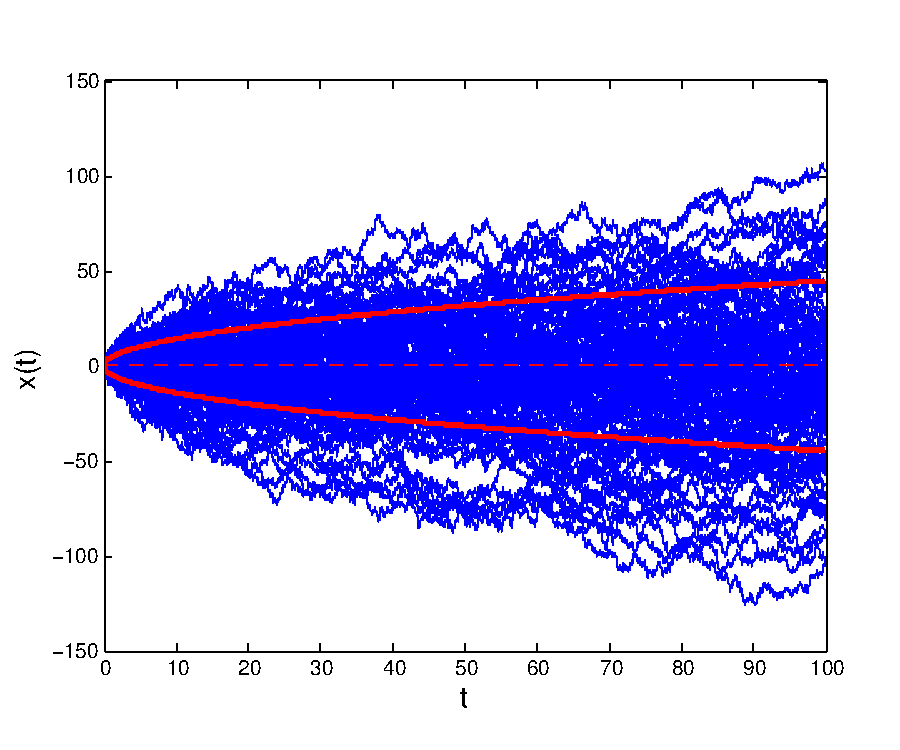
\includegraphics[width=2.5in]{18.Langevin/1d_overdamped_traject.pdf}
		\caption{100 sample trajectories.  The red dashed line and solid lines are the mean $\mean{X}$ and standard deviation
$\sqrt{\mean{X^2}-\mean{X}^2}$, respectively.}
	\label{fig:1d_od_traj}
	\end{subfigure}
	\begin{subfigure}{0.45\textwidth}
		\centering
		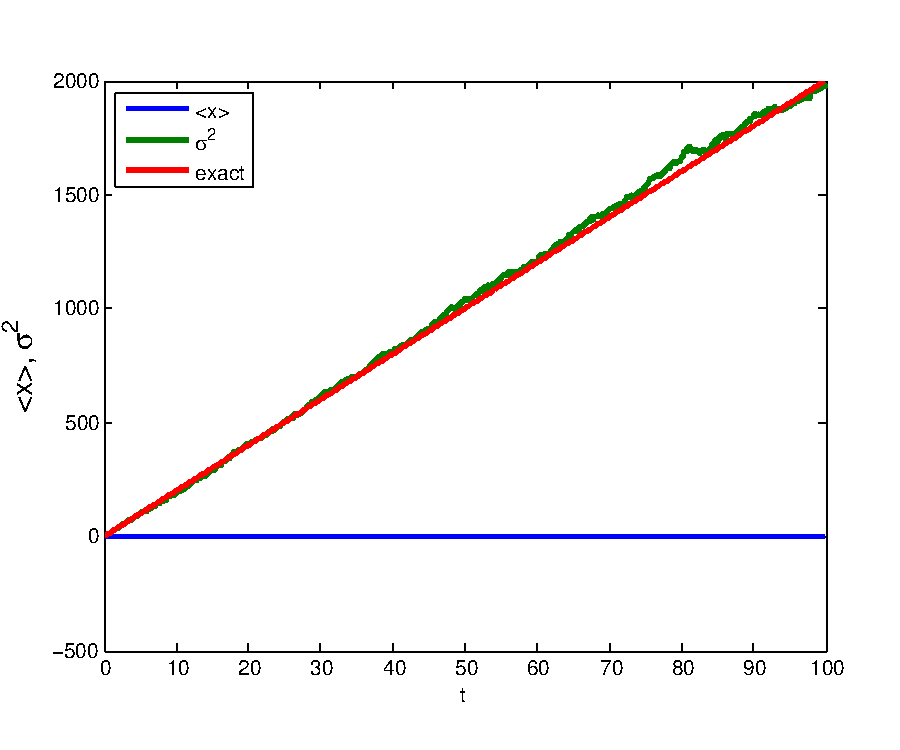
\includegraphics[width=2.5in]{18.Langevin/1d_overdamped_diffusion.pdf}
		\caption{Diffusion. Statistics is taken over 1000 realization. The red line shows the theoretical value $\mean{x^2} = 2 D t$.}
		\label{fig:1d_od_diff}
	\end{subfigure}
\caption{Diffusion of the one-dimensional Brownian motion modeled by the overdamped Langevin equation. Parameter values are $T=1$, $\gamma=0.1$, and thus $D=10$.}
\end{figure}

\begin{figure}
	\centering
	\begin{subfigure}{0.45\textwidth}
		\centering
		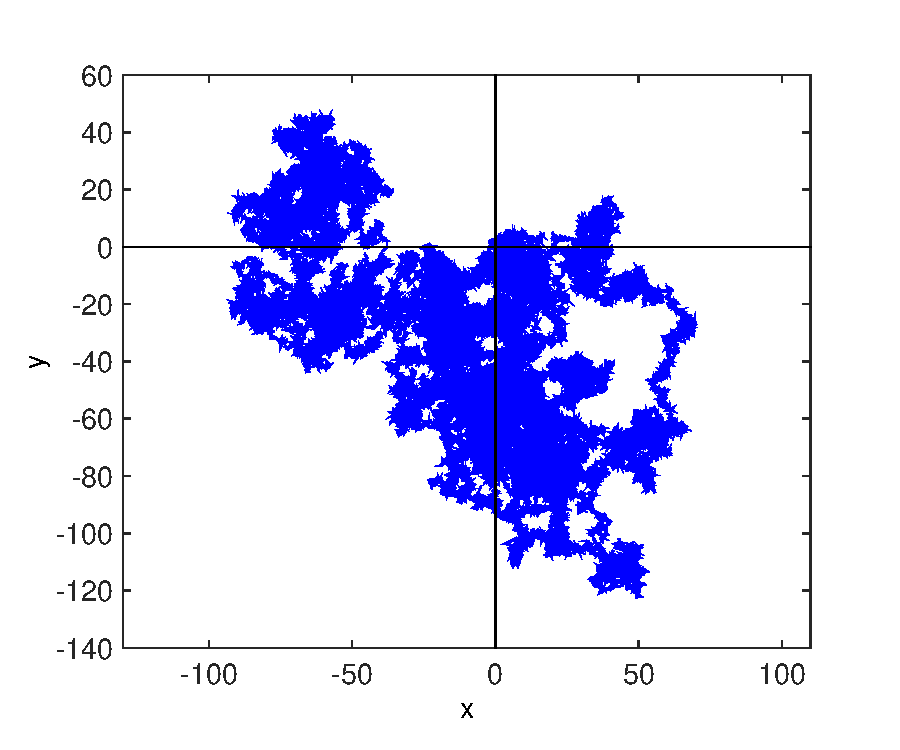
\includegraphics[width=2.5in]{18.Langevin/2d_langevin_traject.pdf}
		\caption{An example of Brownian motion in the two-dimensional space.}
		\label{fig:2d_od_traj}
	\end{subfigure}
	\begin{subfigure}{0.45\textwidth}
		\centering
		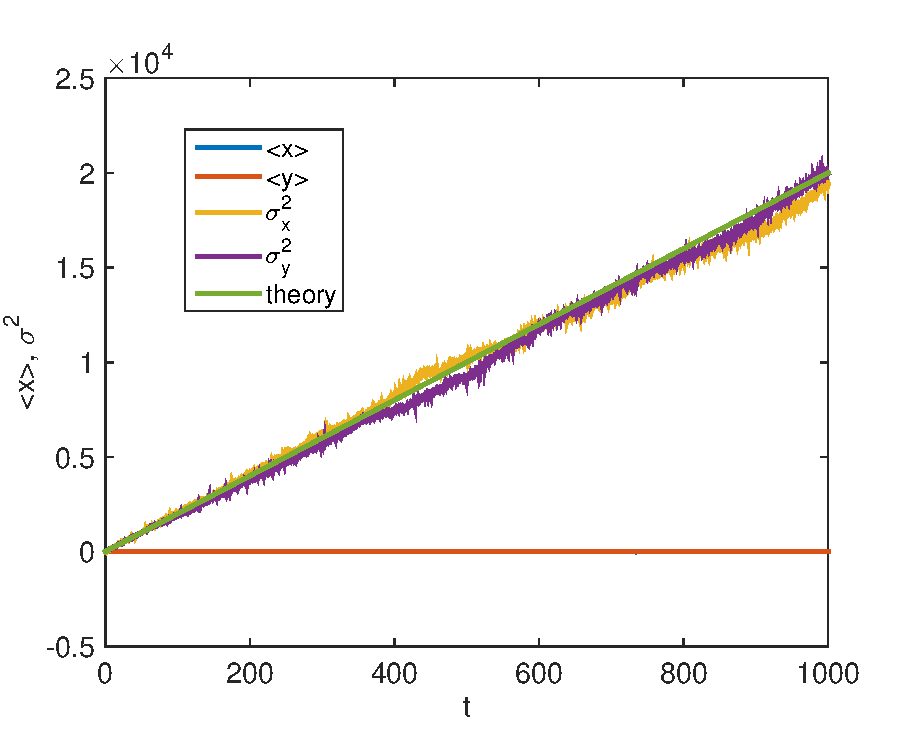
\includegraphics[width=2.5in]{18.Langevin/2d_langevin_diffusion.pdf}
		\caption{Diffusion. Statistics is taken over 1000 realization. The red line shows the theoretical value $\mean{x^2} = 2 D t$.}
		\label{fig:2d_od_diff}
	\end{subfigure}
\caption{Diffusion of the two-dimensional Brownian motion modeled by the overdamped Langevin equations. Parameter values are $T=1$, $\gamma=0.1$, and thus $D=10$.}
\end{figure}

\bigskip
\begin{example}[One-dimensional Wiener process]\label{ex:wiener_1d}

Consider a one-dimensional overdamped Brownian particle freely diffusing in a fluid. The equation of motion for the Brownian particle is the simplest Langevin equation
\begin{equation}\label{eq:1d_od_free}
\dot{X} = \sqrt{2D} \xi(t)
\end{equation}
where $D\kB T/\gamma$. Assuming that the Brownian particle was initially located at $X=0$, we want to find the mean position and the mean square deviation from the mean, i.e., the variance of the particle position, as a function of time.

Program \ref{prog:rw_1d} integrates the Langevin equation (\ref{eq:1d_od_free}) using the Heun method (Algorithm \ref{al:heun_od}) from $t=0$ to $t=100$ with time step $h=0.005$.  Parameter values $\kB T=1$, $\gamma=0.1$, and thus $D=10$, are used.  Figure \ref{fig:1d_od_traj} shows 100 trajectories chosen at random.
The mean position is indicated by the dashed line and the mean deviation $\sigma=\pm \sqrt{\mean{X^2}}$ is plotted with the red solid line.
Despite that all trajectories began at the same point, they are all different.  On the other hand, the mean position remains at $\mean{X}=0$ all time.  The uncertainty of the location increases as time goes.   Figure \ref{fig:1d_od_diff} shows the time evolution of $\sigma^2$. As predicted by
Eq. (\ref{eq:msd_od}),  it increases linearly with time and its slope is $2D=20$.
\end{example}

\newpage
\begin{example}[Brownian motion in two-dimensional space]\label{ex:2d_Brownian}

A Brownian particle is freely diffusion in the two-dimensional space. WE model it using overdamped Langevin equations
\begin{subequations}\label{eq:2d_Brownian}
\begin{eqnarray}
\dot{X} &=& \sqrt{2D} \xi_x(t) \\
\dot{Y} &=& \sqrt{2D} \xi_y(t)
\end{eqnarray}
\end{subequations}
where $\xi_x$ and $\xi_y$ are two independent Gaussian noises defined by 
\begin{equation}
\mean{\xi_i(t)}=0, \quad \mean{\xi_i(t) \xi_j(t')} = \delta_{ij} \delta(t-t'), \quad \forall i,j \in \{x,y\}
\end{equation}
where $\delta_{ij}$ is the Kronecker's delta.

Program \ref{prog:rw_2d} numerically solves Eq (\ref{eq:2d_Brownian}) using the Heun method. Initially the particle was located at the origin of the coordinates and diffuses with $D=10$. Figure \ref{fig:2d_od_traj} illustrates an example trajectory.  The diffusion in $x$ and $y$ directions are independent and each coordinate diffuses in the same way as the one-dimensional Brownian motion as Fig. \ref{fig:2d_od_diff} demonstrates.


\end{example}

\bigskip
\begin{example}[Velocity auto-correlation]

A Brownian particle freely diffusing  is an Ornstein-Uhlenbeck process and mathematically modeled by the Langenvin equation (\ref{eq:ou_v}).  Since the inertial mass plays a role in this case, there is a memory effect. The autocorrelation function of the velocity  (\ref{eq:autocorr_v}) suggests that the correlation time is $\tau_\text{c}=M/\gamma$.  We solve Eq. (\ref{eq:ou_v}) numerically and compute the correlation function.

Program \ref{prog:v_autocorrelation} integrates Eq. \ref{eq:ou_v} 
using the Heun method (Algorithm \ref{al:heun}).  The velocity is calculated from $t=0$ to $t=2^20$ with the time step $\md t=0.002$.  Then the autocorrelation function is computed by FFT (see Section 10.5).  The mass and friction coefficient are assumed to be $M=1$ and $\gamma=0.1$.  Thus, the expected correlation time is $\tau_\text{c}=10$. The result is shown in Figure \ref{fig:v_autocorr}. A sample of stochastic velocity shown in Fig \ref{fig:brownian_velocity} illustrates that the velocity fluctuates around the zero mean.  Since there is no external force, the average velocity should remain zero.  However, due to the random force, the velocity fluctuates around zero.  The velocity looks completely random and there seems no relation between velocity measured at two different time, at least from the naked eye.  However, there is a short time correlation.  The autocorrelation function plotted in Fig \ref{fig:correlation} shows it clearly.  The correlation decays exponentially as expected from Eq. (\ref{eq:autocorr_v}) and  the correlation time appears to be about 10, which agrees with the theoretical value..  It is also noted that up to the correlation time $\tau_\text{c}$, the agreement between the simulation and the exact curve is very good.  Beyond the correlation time, the memory effect phases out and the randomness dominates.  Then, the agreement between the simulation and theory becomes poor since the fluctuation in the correlation becomes larger and more sampling are needed to get a better statistics.
\end{example}


\begin{figure}
	\centering
	\begin{subfigure}{0.45\textwidth}
		\centering
		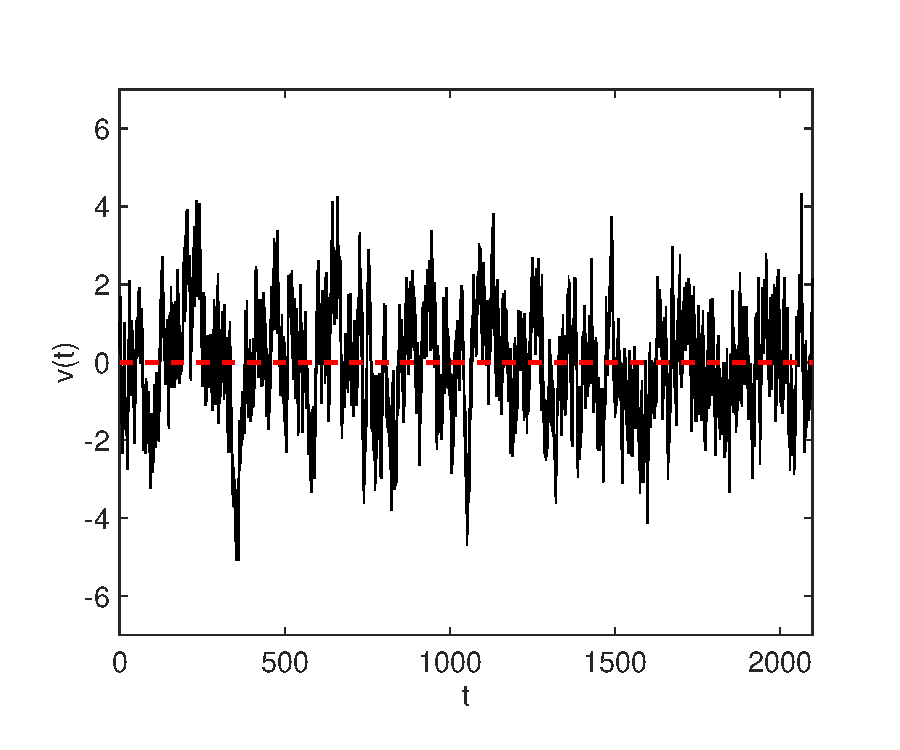
\includegraphics[width=2.5in]{18.Langevin/velocity.pdf}	
		\caption{A fluctuating velocity.}
		\label{fig:brownian_velocity}
	\end{subfigure}
	\begin{subfigure}{0.45\textwidth}
		\centering
		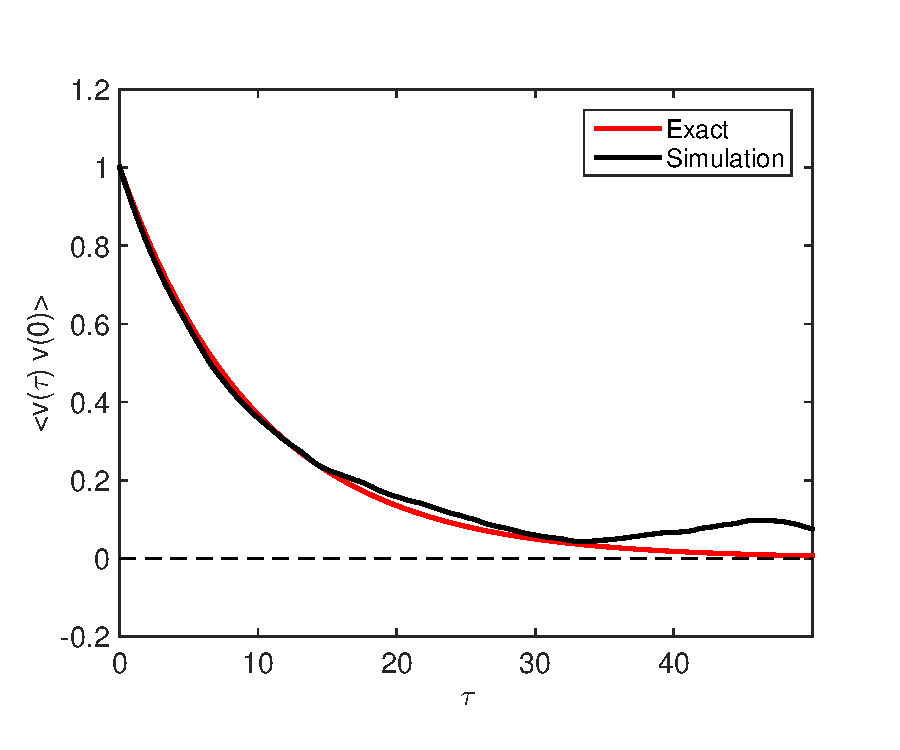
\includegraphics[width=2.5in]{18.Langevin/correlation.pdf}
		\caption{Autocorrelation function of the velocity.  As the result, the agreement becomes poor due to the insufficient statistical sampling.}
		\label{fig:correlation}
	\end{subfigure}
\caption{Ornstein-Uhlenbeck process is simulated with the langevin equation.  The parameter values $M=1$ and $\gamma=0.1$ is used. The theoretical correlation time is $\tau_\text{c}=10$.}
\label{fig:v_autocorr}
\end{figure}


\begin{figure}
	\centering
	\begin{subfigure}{0.32\textwidth}
		\centering
		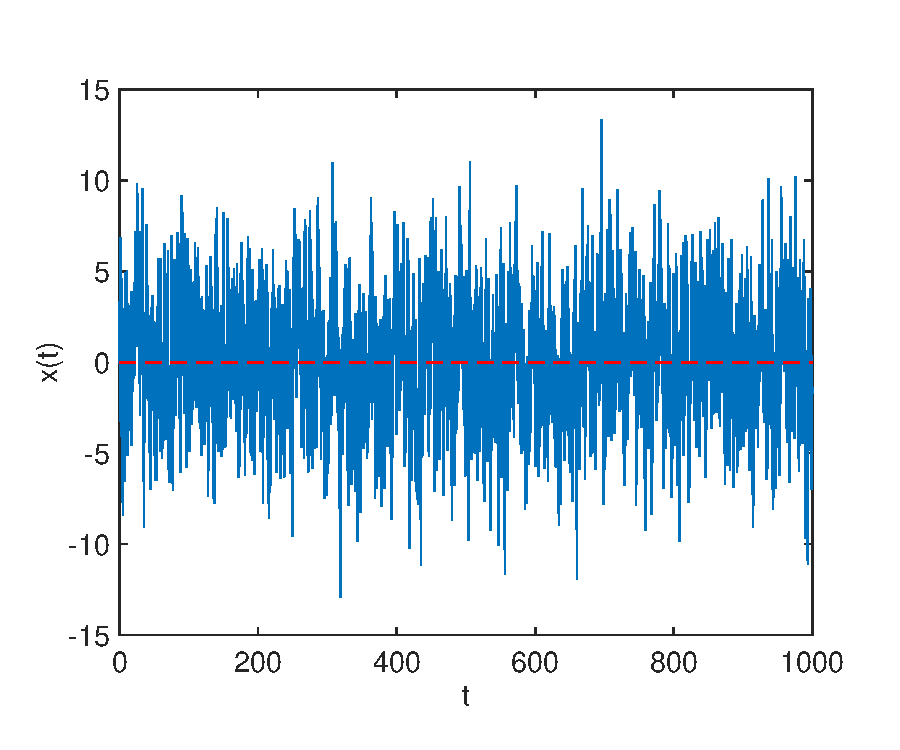
\includegraphics[width=2in]{18.Langevin/Ornstein_Uhlenbeck_traject.pdf}
		\caption{A sample trajectory.  The particle does not stay at the most stable position and fluctuates around the mean position.}
		\label{fig:ou_x_traj}
	\end{subfigure}
	\begin{subfigure}{0.32\textwidth}
		\centering
		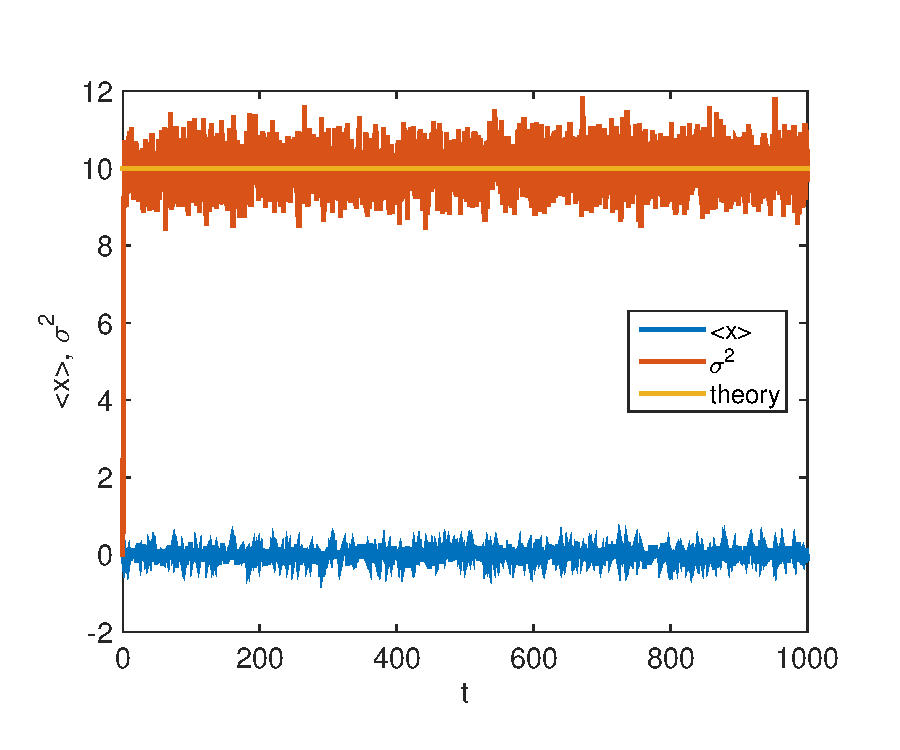
\includegraphics[width=2in]{18.Langevin/Ornstein_Uhlenbeck_stat1.pdf}
		\caption{The mean and the variance sampled over 1000 particles.  The fluscuation is due to the finite sampling.}
		\label{fig:ou_x_stat1}
	\end{subfigure}
	\begin{subfigure}{0.32\textwidth}
		\centering
		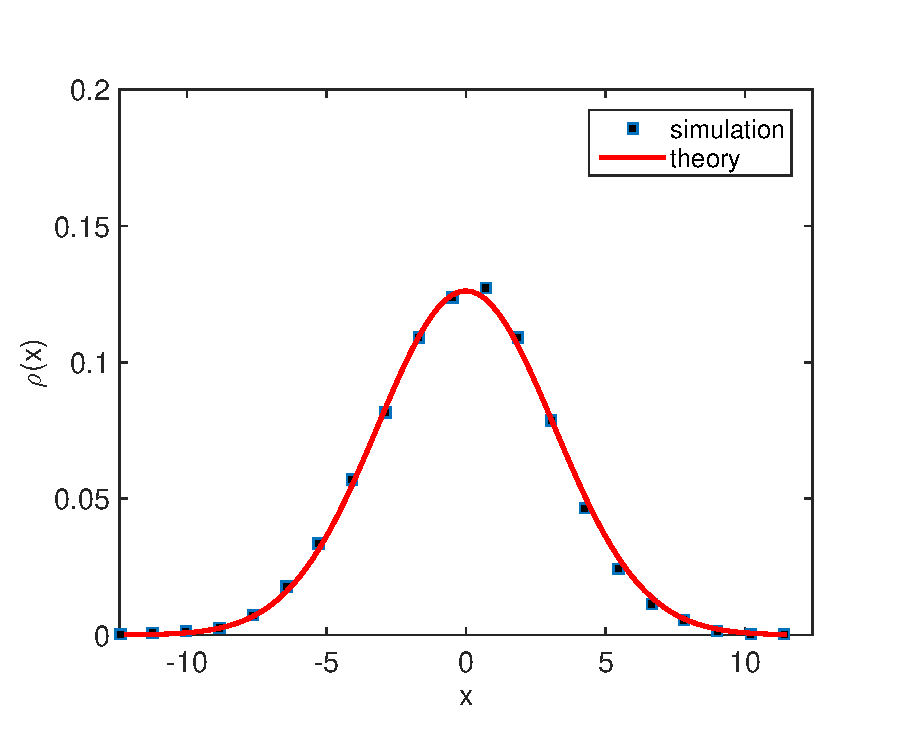
\includegraphics[width=2in]{18.Langevin/Ornstein_Uhlenbeck_stat2.pdf}
		\caption{The probability density of the Brownian particle position. It is Gaussian distributed and agreement with the theory is very good.}
		\label{fig:ou_x_stat2}
	\end{subfigure}
\caption{Brownian harmonic oscillator.  Parameter values $M=1$, $\gamma=0.1$, and $k=1$ are used. The Overdumpled Langevin equation (\ref{eq:ou_x}) is integrated with $\Delta t=0.005$.}\label{fig:brownian_harmo}
\end{figure}

\begin{example}[Brownian Harmonic Oscillators]\label{ex:ou_x}

A Brownian particle of mass $M$ is trapped in harmonic potential $U(x) = \displaystyle\frac{k}{2} x^2$. In a regular classical mechanics course, we learned that the particle eventually settles down at the equilibrium position $x=0$.  When the mass $M$ is very large, that is what happens.   However, when the mass is not so large, the random force kicks the particle all time.  Hence, it cannot dumps out to the resting position. The Brownian particle diffuses around the equilibrium position.

Here the motion of the Brownian particle is modeled by the overdamped Langevin equation (\ref{eq:ou_x}).  This is an Orstein-Uhlenbeck process.
Theoretical analysis suggests that after a certain time, the probability distribution of the particle reaches a steady distribution
\begin{equation}
\rho(X) \propto \me^{-U(X)/\kB T} = \me^{-k X^2/2 \kB T}
\end{equation}
which is a Gaussian distribution with the mean position $\mean{x}=0$ and the mean square displacement $\sigma = \kB T/k$.  Note that unlike the free diffusion, the mean square displacement does not increase.  It remains constant.

We want to confirm this theoretical prediction using a numerical method.
Program \ref{prog:orstein-uhlenbeck} integrates Eq. (\ref{eq:ou_x}) using the Heun method and compare the results with the analytic theory. The parameter values are $M=1$, $\gamma=0.1$, and $k=1$.  The results are plotted in Figures \ref{fig:brownian_harmo}.  First, Fig \ref{fig:ou_x_traj} shows an expmple of the trajectory. Unlike the determinstic overdumpled oscillator, it does not do=ump out to the resting position at $X=0$.  Instead it fluctuates around it due to the random force. Second figure \ref{fig:ou_x_stat1} shows the mean and the variance of the position.  The average is taken over 1000 realizations.  The number of samples is not so large and the instantaneous mean and variance fluctuate significantly.  However, the system is self averaging, meaning that average over time also converges to the same statistical average.  Figure \ref{fig:ou_x_stat2} plots the probability density.  Tahnks to the self-sveraging, the agreement between the simulation and theory is rather good compared to Figure \ref{fig:ou_x_stat1} despite the number of sampling was relatively small.



\end{example}

\noindent
\section{Applications in Physics}

\subsection{Brownian Motors:  Flashing Ratchet}

\begin{figure}
\centering
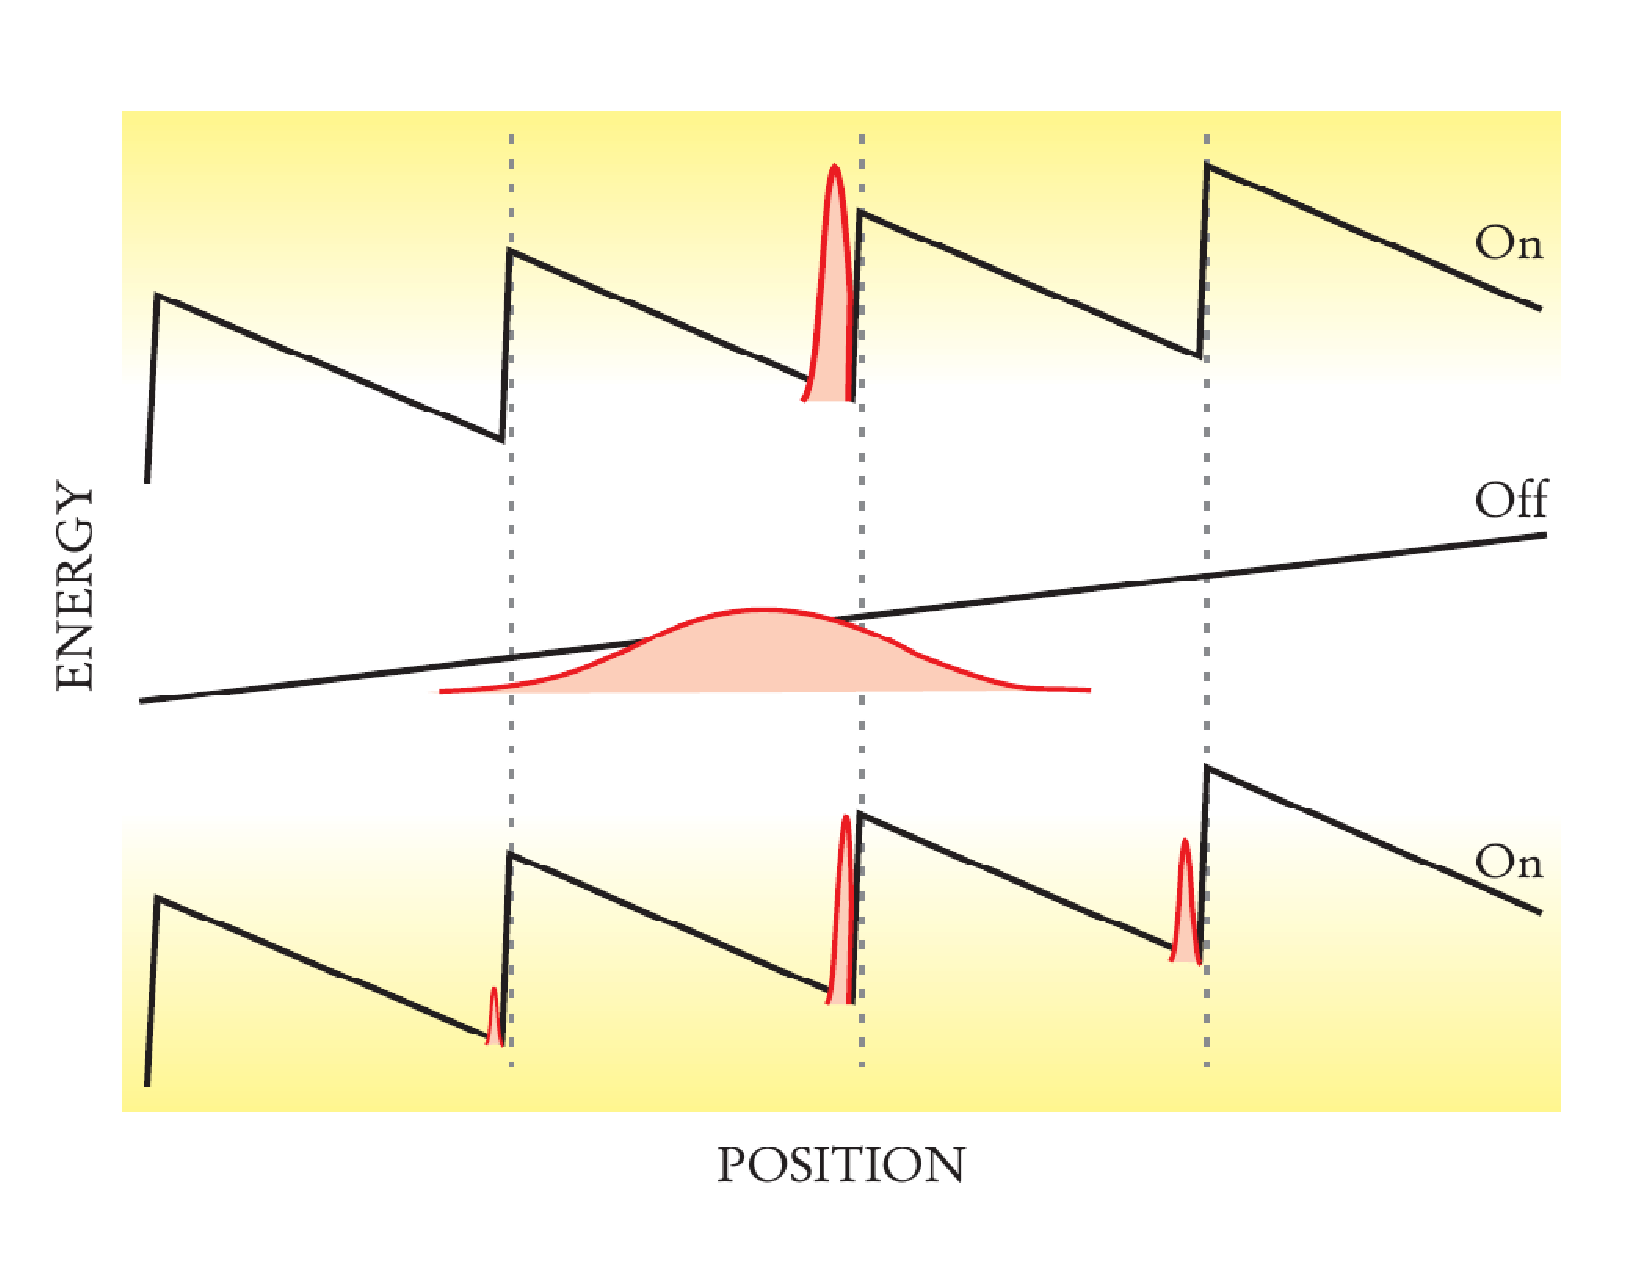
\includegraphics[width=2.5in]{18.Langevin/ratchet.pdf}
\caption{Mechanism of a flashing ratchet. When the potential is on, the particles are localized near the bottom of the potential.  As soon as the potential is turned off, the particles diffuse.  If there is an external force, they also drift (to the left in this setting). By the time when the potential is turned on again, the distribution is wide enough to reach adjacent potential minima.  However, due to the asymmetry in the potential, the chance that the particles go to the right is higher against the external force.  In this model the Brownian particles rectified the thermal fluctuation and move to the right on average.}
\label{fig:flashing_ratchet}
\end{figure}

A regular heat engine extracts energy as heat from the environment and converts it to work.  However, the thermodynamic second law prohibits the conversion of the whole of heat to work.  Some energy must be dumped to another environment at a lower temperature.  Therefore, a heat engine needs to interact with two \textit{heat baths} with different temperature.  In other words, we cannot rectify thermal energy in a single heat bath to drive the heat engine.  That is a common sense of thermodynamics.

However, the laws of thermodynamics do not apply to the systems in non-equilibrium conditions.  It has been shown that it is possible to rectify thermal energy in a single heat bath by creating certain non-equilibrium conditions. It requires to break two symmetries, detailed balance and inversion symmetry ($f(x) \ne f(-x)$.
One example of such a system is a flashing ratchet\cite{ratchet-sciam,ratchet-phystoday} shown in Fig \ref{fig:flashing_ratchet}.
Brownian particles are in a periodic potential with a sawtooth like profile.  Initially, the particles are localized near the bottom of the potential.  The potential is deep enough that thermal fluctuation is small.  Then, the potential is switched off for a while and the particles begin to diffuse freely.  When the potential is back on, the particle slides down to the bottom of the potential.  However, it may not be the same location as they started.  The particles are spread over three minima.  Due to the asymmetry in the potential profile, more particles move to the right.  Hence, on the average the particles move to the right.  Even when a small external force toward the left, the particles still move to the right.  Although there is only one heat bath, the particles are able to move in one direction by rectifying the thermal fluctuation.  This does not violate the second law of thermodynamics since some external source injects energy to the system by switching potential on and off, which breaks the detailed balance.  The asymmetry in the potential profile breaks the inversion symmetry.  We call this ``engine''  a flashing ratchet, which is one kind of Brownian motors.\footnote{Motor proteins such as myosin and kinesin are considered as Brownian motors.}

Program \ref{prog:flashing_ratchet} simulates this Brownian motor with the overdamped Langevin equation.  We use a potential function (see the inset in Fig \ref{fig:ratchet_traject}.)
\begin{equation}\label{eq:ratchet_potential}
U(x) = U_0 \left [ \sin(2 \pi x/L) - \sin(4 \pi x/L)/4 \right ] - x F_\text{ext}
\end{equation}
where $L$ is the period and $U_0$ is a positive constant and $F\_\text{ext}$ is an external constant force.  The  barrier height is about $2U_0$ and the probability that the particles jump over the barrier due to random force is about $\me^{-2U_0/D} = \me^{-2\gamma U_0/\kB T}$.  In order for the ratchet to work, the particles should not jump over the barrier and thus $2 U_0/D > 1$.

Using the parameter values indicated in the caption of Fig. \ref{fig:ratchet_sim}, the particles are clearly moving to the left against the external force.  The mean position plotted in Fig \ref{fig:ratchet_stat} shows that the drift toward the left is steady.

\begin{figure}
	\centering
	\begin{subfigure}{0.45\textwidth}
		\centering
		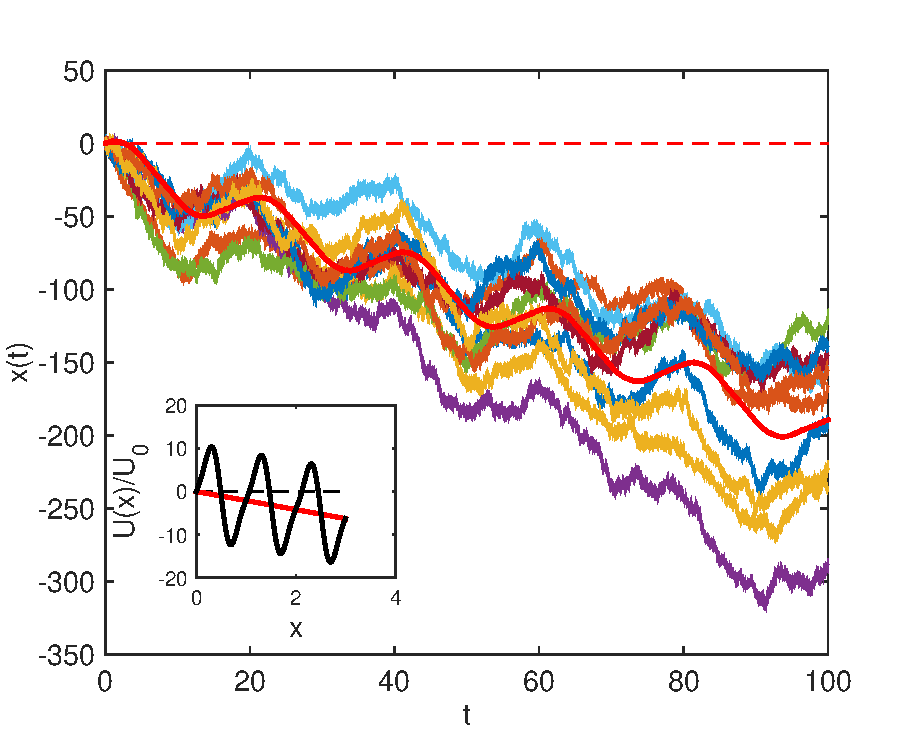
\includegraphics[width=2.3in]{18.Langevin/ratchet_traject.pdf}
		\caption{Sample trajectories.}
		\label{fig:ratchet_traject}
	\end{subfigure}
	\begin{subfigure}{0.45\textwidth}
		\centering
		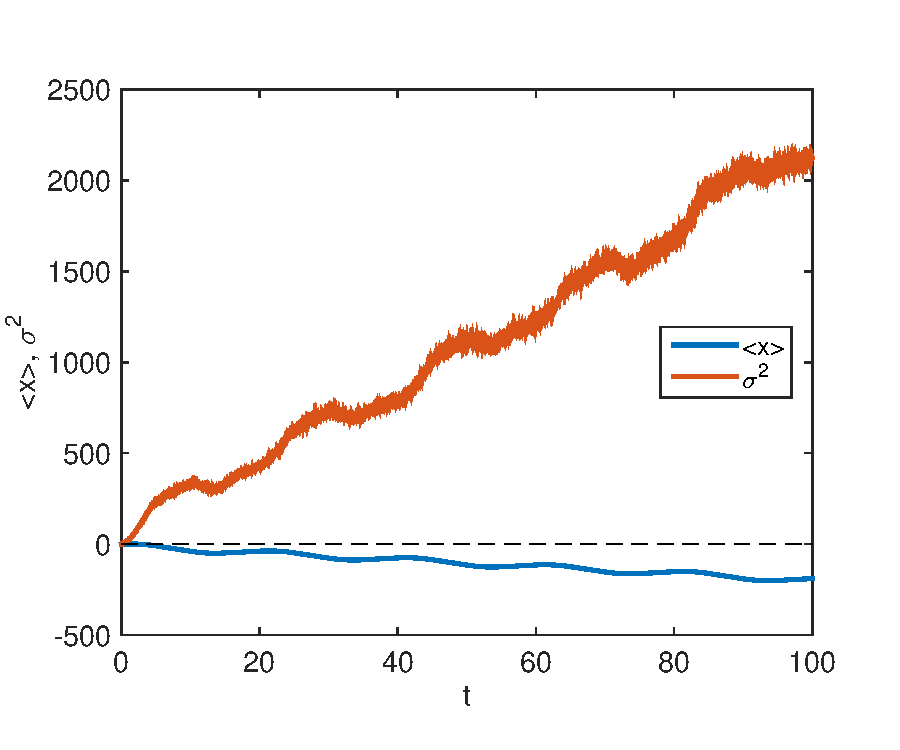
\includegraphics[width=2.3in]{18.Langevin/ratchet_stat.pdf}
		\caption{Mean and variance}
		\label{fig:ratchet_stat}
	\end{subfigure}
\caption{Langevin simulation of the flashing ratchet. The inset in the left panel shows the total potential [Eq. (\ref{eq:ratchet_potential})].  The solid line indicates the potential due to the external force to the right. Parameter values $\kB T=1$, $\gamma=0.1$, $L=1$, $U_0=10$, and $F_\text{ext}=2$ are used.  The corresponding diffusion constant is $D=10$.  The potential is alternatively on for $\tau_\text{on}=10$ and off for $\tau_\text{off}=10$.  The left panel shows that the particles are moving to the left despite that the external force is applied to the right.  The mean position shown in the right panel indicates that the particles move to the left with constant velocity on average.
}
\label{fig:ratchet_sim} 
\end{figure}

\bigskip

\exercise When the external load is too large, the Brownian motor fails as all motors do.  For the parameter values used here, find the stall load where the drift vanishes.




\subsection{Stochastic Resonance}

\begin{figure}
	\centering
	\begin{subfigure}{0.45\textwidth}
		\centering
		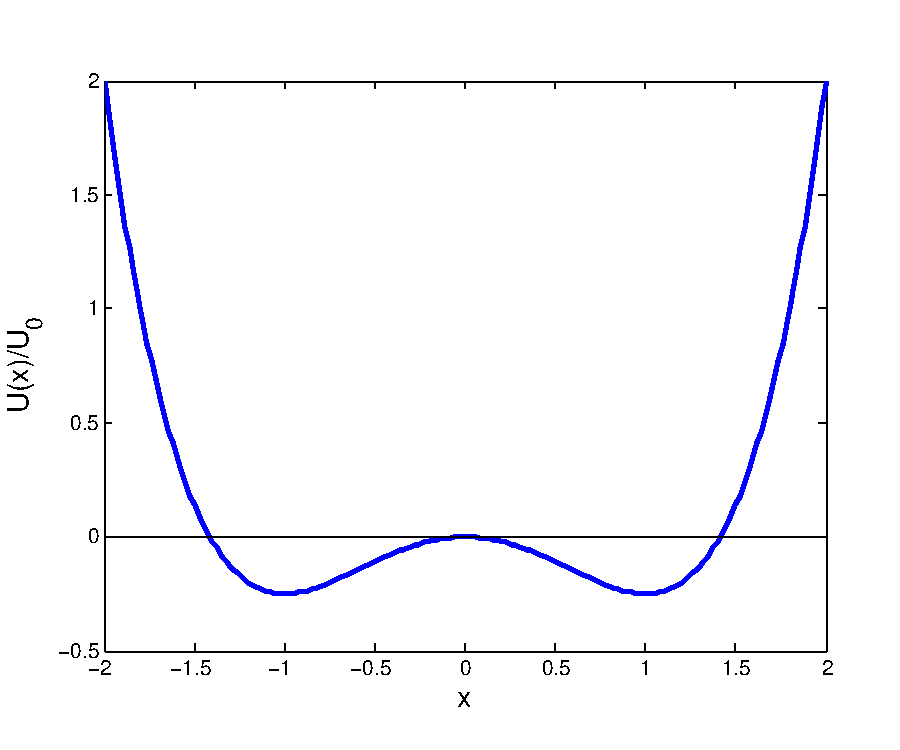
\includegraphics[width=2.5in]{18.Langevin/bistable.pdf}
		\caption{A bistable potential. There are two minimums at $x=\pm 1$ and one maximum at $x=0$.  The potential barrier at $x=0$ has a barrier height $\Delta U = U_0/4$.}
		\label{fig:bistable}
	\end{subfigure}
	\begin{subfigure}{0.45\textwidth}
		\centering
		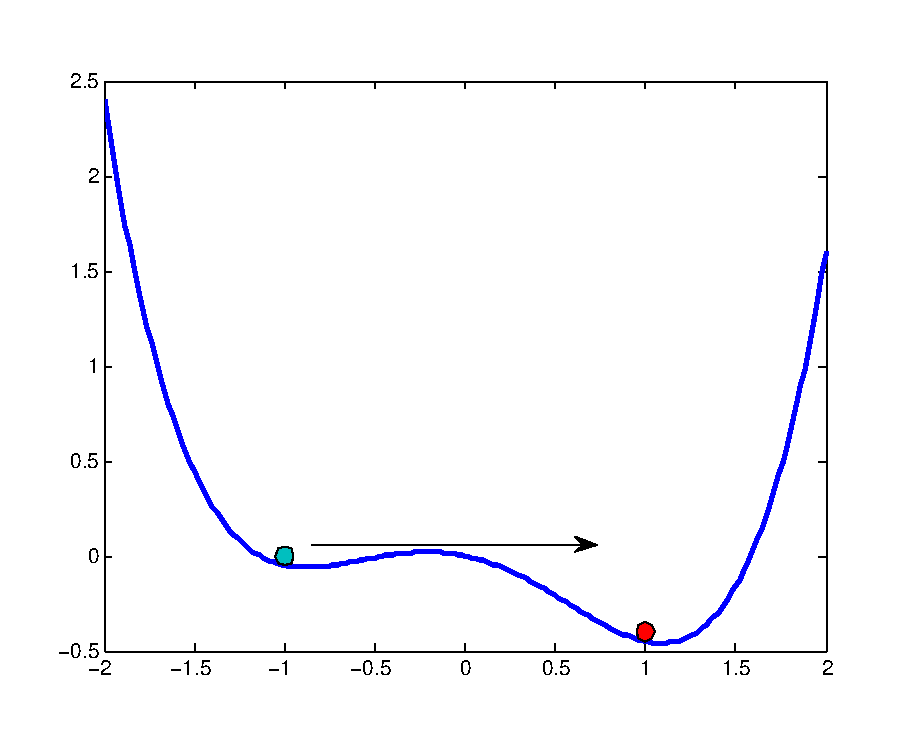
\includegraphics[width=2.5in]{18.Langevin/forced_bistable.pdf}		
		\caption{A bistable potential with a force. An additional potential corresponding to a constant force $F=0.2$ is added to the bistable potential.  A particle in the shallow minimum can easily cross over to the deeper minimum.  However the transition from the deeper side to the shallow side is much more difficult.}
		\label{fig:forced_bistable}
	\end{subfigure}
	\caption{Bistable potentials used in the stochastic resonance model.}
\end{figure}

Consider a bistable potential
\begin{equation}
U(x) = U_0 \left ( \frac{x^4}{4} - \frac{x^2}{2} \right )
\end{equation}
which has two stable points at $x=\pm 1$, See Fig.\ref{fig:bistable}. The height of the potential barrier separating two minimums is
$\Delta U = U_0/4$. Suppose that a Brownian particle is trapped in the left side of potential.  Due to the thermal fluctuation, there is a chance that the particle crosses the barrier to the right side.  The transition rate is proportional to $\me^{-\Delta U/\kB T}$. Therefore, when $\kB T \ll \Delta U$, the particle stays in one side for a long time.  On the other hand, when $\kB T \gg \Delta U$, the particle can move between two minimums almost freely.  When $\kB T \sim \Delta U$, the particle stays in one side for a while and jumps to the other side and stays there for a certain time. Then, come back again.  This is a kind of oscillator.  However, the jump happens at random and there is no clear period.

When a constant force $F>0$ is applied, the potential loses the symmetry and one side becomes deeper than the other as illustrated in Fig \ref{fig:forced_bistable}.  When the force is weak, the barrier height from the shallow minimum is $\Delta U_- = -U_0/4+F$ and the other barrier height is $\Delta U_+ = -U_0/4-F$.  If temperature is chosen so that $\Delta U_+ > \kB T > \Delta U_+$, then the particle in the shallower minimum easily jumps over to the deeper minimum.  On the  other hand, the particle in the deeper minimum stays in the deeper minimum for a long time.

Now we apply a locking force
\begin{equation}
F(t) = A \cos(\Omega t)
\end{equation}
where $A$ and $\Omega$ are an amplitude and frequency.  We regard this force as an input signal.  The output signal is the motion of the Brownian particle.   We assume that $A < 2 U_0 /3 \sqrt{3}$ so that the potential barrier exist.  When temperature is sufficiently low (low noise), the particle tends to stay in one side. Therefore, information of the input signal is lost.  When temerature is too high, the particle jumps between two minimum randomly and thus the input signal is lost again.   If an appropriate noise intensity is used, the particle moves toward the deeper minimum and oscillates between the minima as the force rocks back and forth.  The input signal is retained only when the noise intensity is right.  This phenomena is known as stochastic resonance.  You can tune into the input frequency by adjusting the strength of the noise.  This is counter intuitive since noises usually destroy the signal.

We model this process using the overdamped Langevin equation
\begin{equation}
\dot{X} = -U'(X) + A \cos(\Omega t) + \sqrt{2D} \xi(t)
\end{equation}
inplimented in Program \ref{prog:stochastic_resonance}.
The parameter values $U_0=10, A=1, \Omega=0.5$ are fixed.  Then, we very the noise intensity $D$.  In Fig. \ref{fig:sr}, three different cases, weak noise, $D=0.5$ (left panel), resonant noise $D=1.2$ (center panel), and strong noise, $D=2.0$ (right panel).  When the noise is too week, the particle stay in the same side for a long time and occasionally jumps to the other side.  It is not following the input signal.  
On the other hand, the strong noise causes rapid random jumps and again it is not following the input signal.  when the noise intensity takes an appropriate value, the Brownian particle follows the input signal.  The power spectrum of the trajectories are plotted in the lower panel.
When the stochastic resonance occurs, the spectrum clearly shows a peak at $\omega=\Omega$ and thus the trajectory and the signal have the same periodic motion.  The two other cases do not have such a peak.

\begin{figure}
	\begin{subfigure}{0.32\textwidth}
		\centering
		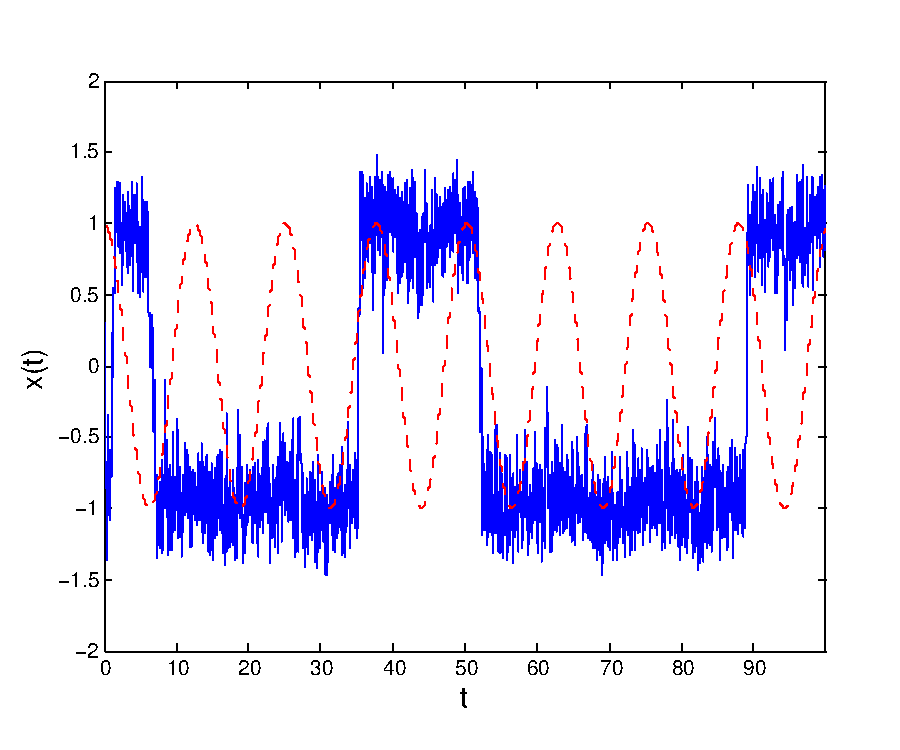
\includegraphics[width=2in]{18.Langevin/sr_low.pdf}
		\caption{}\label{fig:sr_l}
	\end{subfigure}
	\begin{subfigure}{0.32\textwidth}
		\centering
		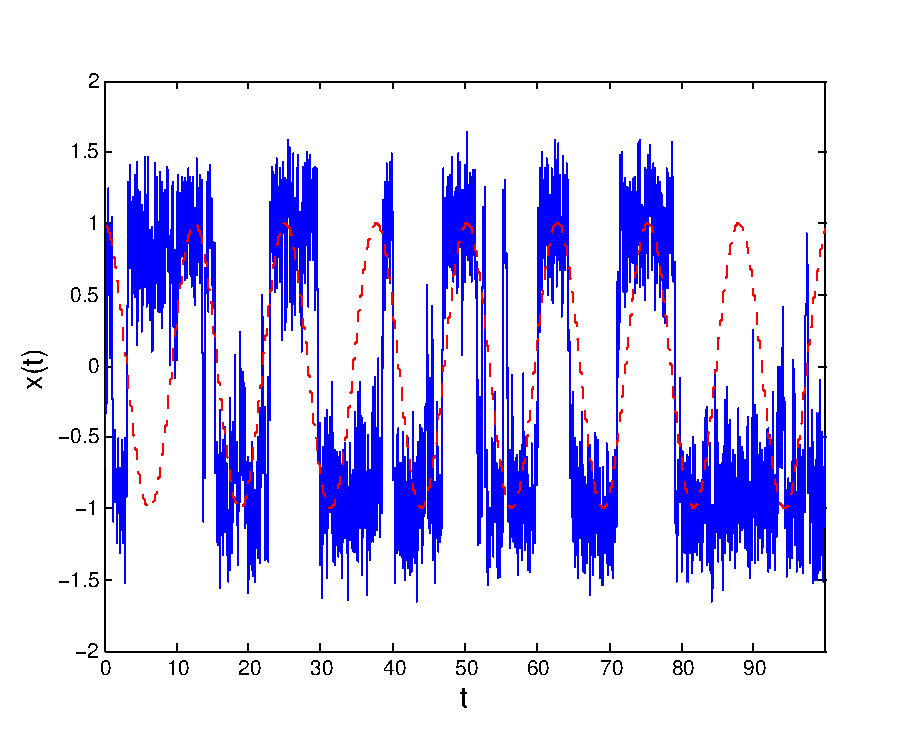
\includegraphics[width=2in]{18.Langevin/sr_match.pdf}
		\caption{}\label{fig:sr_m}
	\end{subfigure}
	\begin{subfigure}{0.32\textwidth}
		\centering
		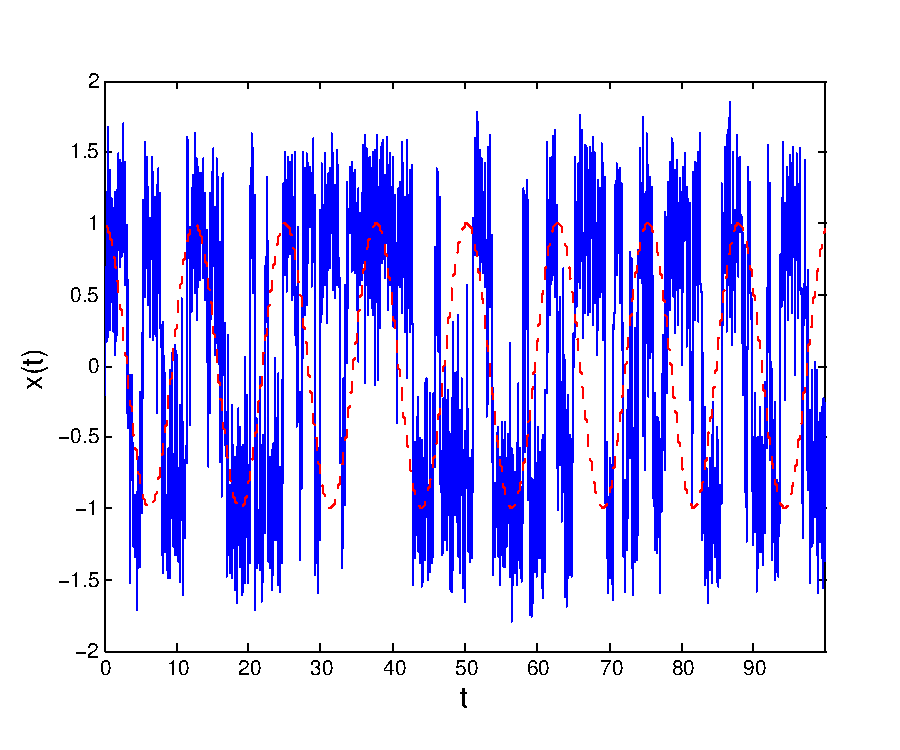
\includegraphics[width=2in]{18.Langevin/sr_high.pdf}
		\caption{}\label{fig:sr_h}
	\end{subfigure}
//
	\begin{subfigure}{0.32\textwidth}
		\centering
		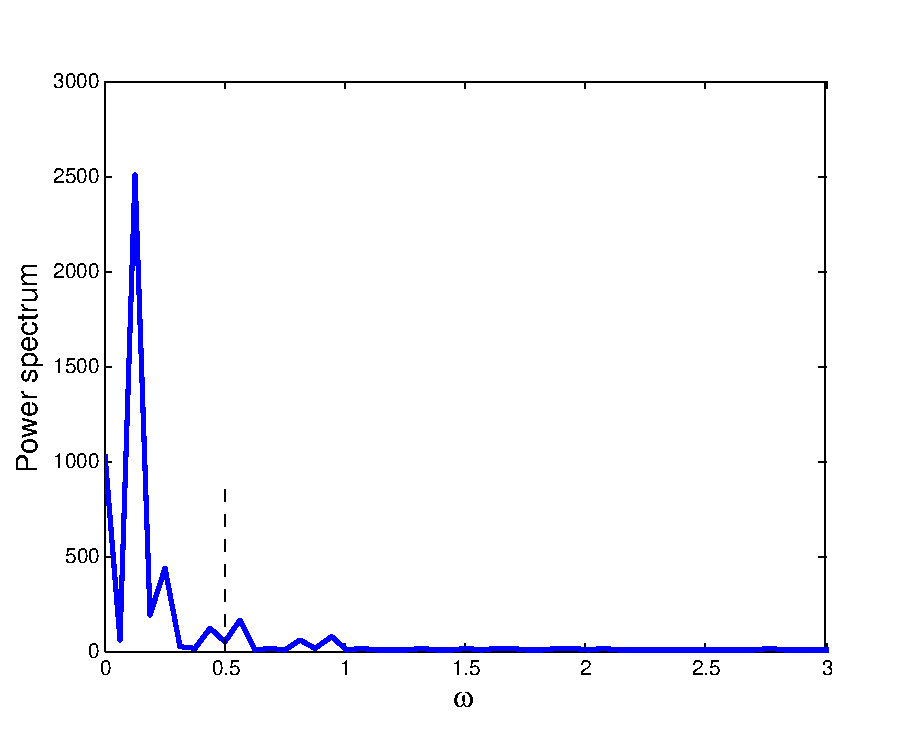
\includegraphics[width=2in]{18.Langevin/sr_low_spectrum.pdf}
		\caption{}\label{fig:sr_l_spec}
	\end{subfigure}
	\begin{subfigure}{0.32\textwidth}
		\centering
		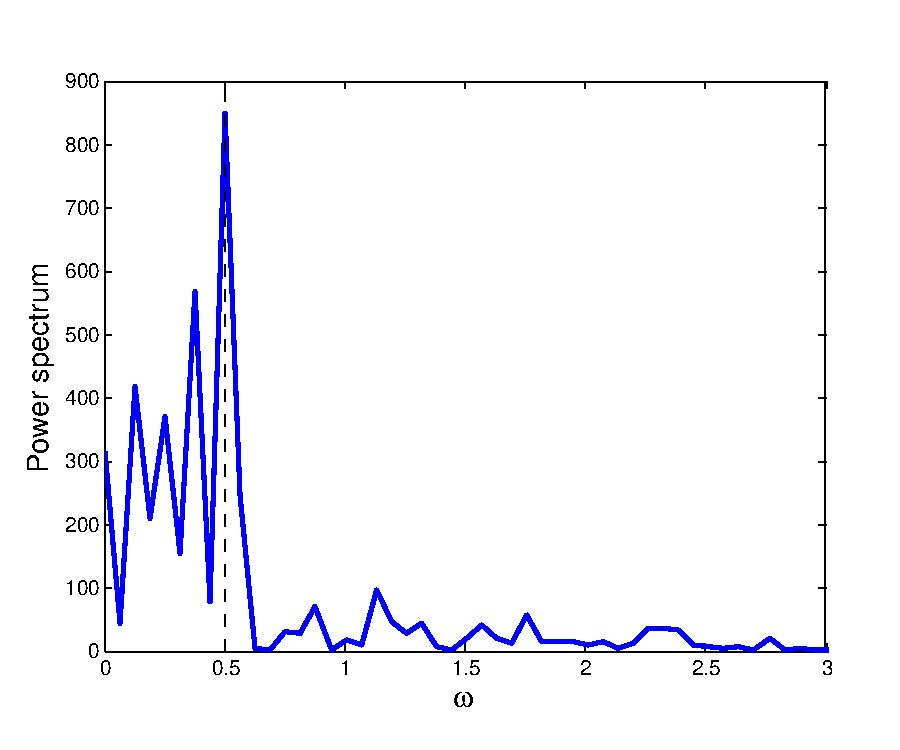
\includegraphics[width=2in]{18.Langevin/sr_match_spectrum.pdf}
		\caption{}\label{fig:sr_m_spec}
	\end{subfigure}
	\begin{subfigure}{0.32\textwidth}
		\centering
		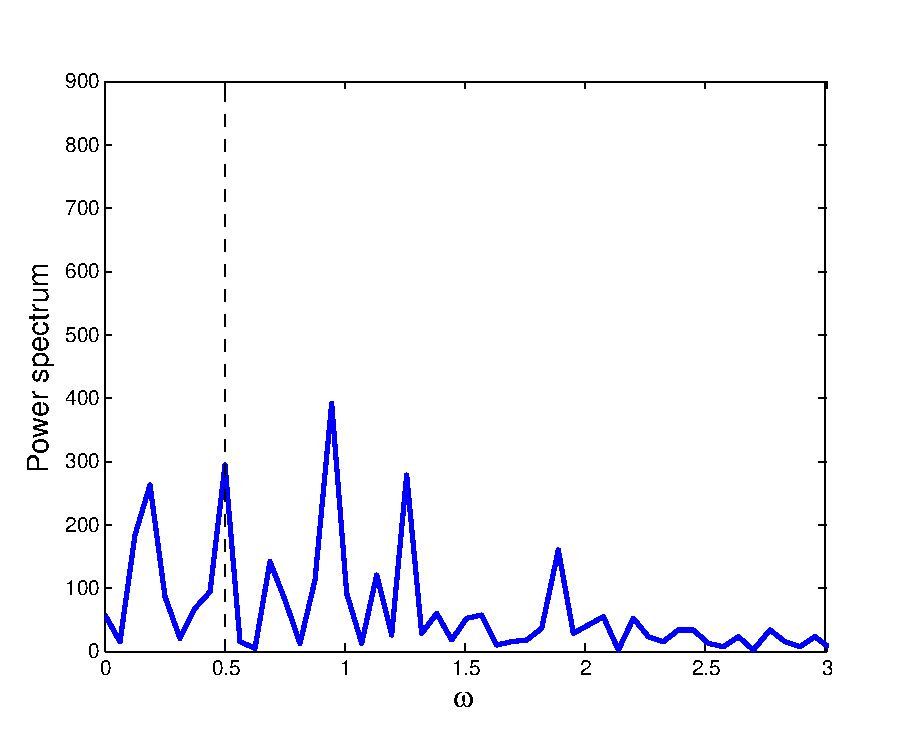
\includegraphics[width=2in]{18.Langevin/sr_high_spectrum.pdf}
		\caption{}\label{fig:sr_h_spec}
	\end{subfigure}
\caption{Stochastic Resonance. The upper panels show the trajectories of the Brownian particle and the lower panels plot the power spectrum of the corresponding trajectories.  Parameter values $U_0=10, A=1, \Omega=0.5$ are fixed.  There different noise intensity, $D=0.5$ (left), $D=1.2$ (center) and $D=2.0$ (right) are used.  The trajectory in the center panel shows that the Brownian particle roughly flows the input signal.  The power spectrum clearly shos a peak at $\omega=\Omega$, indicating that the input and output signals are in resonance.}
\label{fig:sr}
\end{figure}

The stochastic resonance is originally introduced to explain the periodic recurrences of the ice ages.\cite{sr_wiesenfeld,sr_bulsara}   SInce then, it has been demonstrated in variety of physical systems including laser systems.  It is also widely spread in biology  for an example sensory systems.  Now it is observed in network.  It became a most poplar noise induced phenomena.

newpage
\noindent
\section{Problems}

\begin{enumerate}[labelwidth=0.5cm,labelindent=0cm,leftmargin=*,label=\bfseries \thechapter.\arabic*,align=left]
\item
In Example \ref{ex:ou_x}, we investigated the Brownian particles in a harmonic potential.  The motion of the Brownian particles is the Orstein-Uhlenbeck process.  Using the same parameter values and the same initial condition, evaluate the mean square displacement as a function of time and compare the results with the analytic solution
\begin{equation}
 \mean{X(t)^2}-\mean{X(t)}^2 = \frac{\kB T}{k} \left [ 1 - \me^{-2 k t /\gamma} \right ]  
\end{equation}

\end{enumerate}

\newpage
\noindent
\section*{MATLAB Source Codes}
\addcontentsline{toc}{section}{\protect\numberline{}MATLAB Source Codes}

\noindent
\program
\label{prog:rw_1d}
\footnotesize
\begin{verbatim}
%**************************************************************************
%*     Exercise 18.1                                                      *
%*     filename: ch18pr01.m                                               *
%*     program listing number: 18.1                                       *
%*                                                                        *
%*     This program simulates the one-dimensional free continuous-time    *
%*     random walk (Wiener process) using the Heun method.                *
%*                                                                        *
%*     Programed by Ryoichi Kawai for Computational Physics Course.       *
%*     Last modification:  03/25/2017.                                    *
%**************************************************************************
close all
clc

% system parameters
gamma=0.1; % friction coefficient
T=1.0; % temperature

% control parameter
tau=100;  % total duration
dt=0.005; % time step
D=T/gamma;  % diffusion constant
ds=sqrt(2.0*D*dt); % time step for Wiener process
N=int32(tau/dt);  % number of steps
M=1000; %number of samplings
t=linspace(0.0,double(N*dt),N+1);

figure(1)
theory=2.0*T/gamma*t; % theoretical variance
p=plot([t(1),t(N+1)],[0,0],'--');
set(p,'color','red')
p=plot(t,sqrt(theory),t,-sqrt(theory));
set(p,'color','red','linewidth',2)
xlabel('t','fontsize',14)
ylabel('x(t)','fontsize',14)
hold on

% reset to zero
sumx1=zeros(N+1,1);
sumx2=zeros(N+1,1);
x=zeros(N+1,1);

% loop over M samplings
for j=1:M
    % initial condition
    x(1)=0;
    % random force with Gaussian stribution
    g=randn(N,1);  

    % solving Langevin equation
    for i=1:N
        x(i+1) = x(i)+g(i)*ds;
    end
    if j<11
        plot(t,x)
        drawnow
    end
    
    % save the data for statistical analysis
    sumx1(:) = sumx1(:)+x(:);
    sumx2(:) = sumx2(:)+x(:).^2;
end

hold off

% statistical analysis
xmean=sumx1./M;   % <x>
sumx2=sumx2./M;   % <x^2>
xvar=sumx2-xmean.^2;  % variance

figure(2)
p=plot(t,xmean,t,xvar,t,theory)
set(p,'linewidth',2)
xlabel('t');
ylabel('<x>, \sigma^2','fontsize',14)
legend('\langle x \rangle','\sigma^2','exact')
legend('location','northwest')
hold off
\end{verbatim}
\normalsize

\noindent
\program
\label{prog:rw_2d}
\footnotesize
\begin{verbatim}
%**************************************************************************
%*     Exercise 18.2                                                      *
%*     filename: ch18pr02.m                                               *
%*     program listing number: 18.2                                       *
%*                                                                        *
%*     This program simulates the two-dimensional free continuous-time    *
%*     random walk (Wiener process) using the Heun method.                *
%*                                                                        *
%*     Programed by Ryoichi Kawai for Computational Physics Course.       *
%*     Last modification:  03/25/2017.                                    *
%**************************************************************************
close all
clc

% system parameters
gamma=0.1;  % frictional constant
T=1.0;      % temperature  
D=T/gamma;  % strength of noise

% control parameter
tau=100; % total time
dt=0.005; % time step
ds=sqrt(2.*D*dt); % Wiener step size
N=ceil(tau/dt); % number of steps
t=linspace(0.0,double(N*dt),N+1);
M=100; % number of samples

% reset the counters
sumx1=zeros(N+1,1);
sumx2=zeros(N+1,1);
sumy1=zeros(N+1,1);
sumy2=zeros(N+1,1);
x=zeros(N+1,1);
y=zeros(N+1,1);

% sampling loop begins
for j=1:M
    
    x(1)=0; % initial position
    y(1)=0;
    
    % Normally ditributed random numbers by the Box-Muller method
    g=randn(N,2);

    % integration of the Langevin equation
    for i=1:N
        x(i+1) = x(i)+g(i,1)*ds;
        y(i+1) = y(i)+g(i,2)*ds;
    end
    
    % record the data for statistical analysis
    sumx1 = sumx1+x;
    sumy1 = sumy1+y;
    sumx2 = sumx2+x.^2;
    sumy2 = sumy2+y.^2;
end

% plot a sample trajectory
figure(1)
plot(x,y)
hold on
plot(x(1),y(1),'.','color','Red')
axis equal;
xlabel('x','fontsize',14)
ylabel('y','fontsize',14)
hold off

% statistical analysis
figure(2);
xmean=sumx1/M;   % <x>
ymean=sumy1/M;   % <y>
sumx2=sumx2/M;   % <x^2>
sumy2=sumy2/M;   % <y^2>
xvar=sumx2-xmean.^2; % variance_x
yvar=sumy2-ymean.^2; % variance_y
theory=2*T/gamma*t;  % theoretical variance
p=plot(t,xmean,t,ymean,t,xvar,t,yvar,t,theory);
set(p,'linewidth',2)
xlabel('t','fontsize',14)
ylabel('<x>, \sigma^2','fontsize',14)
legend('<x>','<y>','\sigma_x^2','\sigma_y^2','theory')
legend('location','east')
\end{verbatim}
\normalsize

\noindent
\program
\label{prog:v_autocorrelation}
\footnotesize
\begin{verbatim}
%**************************************************************************
%*     Exercise 18.3                                                      *
%*     filename: ch18pr03.m                                               *
%*     program listing number: 18.3                                       *
%*                                                                        *
%*     This program calculates temporal autocorrelation of velocity of    *
%*     one-dimensional Brownian particles.                                *
%*                                                                        *
%*     Programed by Ryoichi Kawai for Computational Physics Course.       *
%*     Last modification:  03/26/2017.                                    *
%**************************************************************************
close all
clc

% system parameters
m=1;  % mass
gamma=0.1/m; % friction
T=2; % temperature
w=sqrt(2*gamma*T)/m;

% control parameters
N=2^20; % number of data points
dt=0.01;
ds=sqrt(dt)*w;

% initial conditions
x(1)=0; % initial position
v(1)=1; % initial velocity

% random number
g=randn(N,1);

% solve Langevin Eq.
for i=1:N-1
    % Euler step
    x(i+1)=x(i)+v(i)*dt;
    v(i+1)=v(i)-gamma*v(i)*dt+g(i)*ds;
    %Heun step
    x(i+1)=x(i)+(v(i)+v(i+1))*dt/2;
    v(i+1)=v(i)-gamma*(v(i)+v(i+1))*dt/2+g(i)*ds;
end

% velocity autocorrelation
z=fft(v);
y=abs(z).^2;
vc=ifft(y)/N;
vc=vc/vc(1);
t=[0:N-1]*dt;
vx=exp(-gamma*t);

subplot(1,2,1)
p=plot(t,v);
hold on
p=plot([1,t(N)],[0,0],'--');
set(p,'color','red')
xlabel('t','fontsize',14)
ylabel('v(t)','fontsize',14)
axis([t(1) t(N) -7 7])
hold off

subplot(1,2,2)
nc=floor(50/dt);
p=plot(t(1:nc),vx(1:nc));
set(p,'linewidth',2,'color','red')
hold on
p=plot(t(1:nc),vc(1:nc));
set(p,'linewidth',2)
legend('Exact','Simulation');
legend('location','northeast')
xlabel('\tau','fontsize',14)
ylabel('<v(\tau) v(0)>','fontsize',14)
axis([0 t(nc) -0.2 1.2])
p=plot([0,t(nc)],[0,0],'--');
set(p,'color','black')
hold off
\end{verbatim}
\normalsize

\noindent
\program
\label{prog:orstein-uhlenbeck}
\footnotesize
\begin{verbatim}
%**************************************************************************
%*     Example 18.4                                                       *
%*     filename: ch18pr04.m                                               *
%*     program listing number: 18.4                                       *
%*                                                                        *
%*     This program simulates the Orstein-Uhlenbeck process.              *
%*                                                                        *
%*     Programed by Ryoichi Kawai for Computational Physics Course.       *
%*     Last modification:  03/26/2017.                                    *
%**************************************************************************
clear all
clc

% system parameters
gamma=0.1; %friction
T=1.0; %temperature
k=1.0; %spring constant

% control parameter
tau=1000;
dt=0.01;
ds=sqrt(2*T/gamma*dt);
dk=k*dt;
N=ceil(tau/dt); % numner of time steps
M=1000; %number of realization

t=(0:N-1)*dt;

sumx1=zeros(N,1);
sumx2=zeros(N,1);

for j=1:M
    
    x(1)=0;  % initial position
    r=rand(N,2);                                 % Gaussian random numner
    g = sqrt(-2*log(r(:,1))).*cos(2*pi*r(:,2));  % by the Box-Muller

    for i=2:N
        t(i)=(i-1)*dt;
        x(i) = x(i-1)+ds*g(i) - dk*x(i-1);  % Eulrer step
        x(i) = x(i-1)+ds*g(i) - dk*(x(i)+x(i-1))/2;  % Huen step
    end
    sumx1(:) = sumx1(:)+x(:);
    sumx2(:) = sumx2(:)+x(:).^2;
    
end

figure(1);
plot(t,x)
hold on
p=plot([0,t(N)],[0,0],'--');
set(p,'color','red')
xlabel('t','fontsize',14)
ylabel('x(t)','fontsize',14)
hold off

figure(2);
xmean=sumx1./M;
sumx2=sumx2./M;
sigma2=sumx2-xmean.^2;
theory = T/gamma;
p=plot(t,xmean,t,sigma2,[t(1),t(N)],[theory,theory]);
set(p,'linewidth',2)
xlabel('t','fontsize',14)
ylabel('<x>, \sigma^2','fontsize',14)
legend('<x>','\sigma^2','theory')
legend('location','east')

figure(3)
[f,z]=hist(x,21);
dz=z(2)-z(1);
s=sum(f)*dz;
f=f/s;
y0=z(1);
y1=z(end);
y=[1:100]*(y1-y0)/100;
y=y+y0;
h=sqrt(gamma/(2*pi*T))*exp(-k*y(:).^2*gamma/(2*T));
p=plot(z,f,'s',y,h);
xm=max(abs(z(:)));
set(p(1),'MarkerFaceColor','black')
set(p(2),'color','red','linewidth',2)
legend('simulation','theory')
xlabel('x','fontsize',14)
ylabel('\rho(x)','fontsize',14)
axis([-xm xm 0 0.2])
\end{verbatim}
\normalsize


\noindent
\program
\label{prog:flashing_ratchet}
\footnotesize
\begin{verbatim}
%**************************************************************************
%*     Section 18.2.1                                                     *
%*     filename: ch18pr05.m                                               *
%*     program listing number: 18.5                                       *
%*                                                                        *
%*     This program simulates a flashing ratchet.                         *
%*                                                                        *
%*     Programed by Ryoichi Kawai for Computational Physics Course.       *
%*     Last modification:  03/26/2017.                                    *
%**************************************************************************
close all
clear all

% system parameters
gamma=0.1; %friction
T=1; % temperature
L=1; % periodicity
k=2*pi/L; % wave number
U0=10; % potential strength
F0=U0*pi/L; % force strength
Fx=2;  %external load
h=10; % pontential on-off period
D=T/gamma; %noise strength

% control parameter
tau=100;  % total time
dt=0.005;  % time step
ds=sqrt(2.0*D*dt);  % Wiener time step
N=ceil(tau/dt);  % number of iterations
M=1000;

% prepare the arrays
sumx1=zeros(1,N);
sumx2=zeros(1,N);
t=linspace(0,dt*(N-1),N);
x=zeros(1,N);

figure(1)
for j=1:M
    u=0;
    potential=true;
    
    x(1)=0; % initial position
    g=randn(1,N);  % generate Gaussian white noise
    
    for i=1:N-1
        u=u+dt;
        if potential  % diffusion inside the potential
            f1 = -F0*(2.0*cos(k*x(i))-cos(2.0*k*x(i)))+Fx;
            x(i+1) = x(i)+g(i)*ds + f1*dt;
            f2 = -F0*(2.0*cos(k*x(i+1))-cos(2.0*k*x(i+1)))+Fx;     
            x(i+1) = x(i)+g(i)*ds + (f1+f2)*dt/2.0;
        else  % free diffusion
            x(i+1) = x(i)+g(i)*ds+Fx*dt;
        end    
        if u>h
            potential = not(potential);
            u=0;
        end
    end
    if j < 11  % show only 10 trajectories
        plot(t,x)
        drawnow
        hold on
    end
    sumx1 = sumx1+x;
    sumx2 = sumx2+x.^2;
    
end

% statstical analysis
xmean=sumx1./M;
sumx2=sumx2./M;
sigma2=sumx2-xmean.^2;

p=plot([0,t(N)],[0,0],'--');
set(p,'color','red')
p=plot(t,xmean);
set(p,'color','red','linewidth',2)
xlabel('t','fontsize',14)
ylabel('x(t)','fontsize',14)
hold off

figure(2);
p=plot(t,xmean,t,sigma2);
set(p,'linewidth',2)
xlabel('t','fontsize',14)
ylabel('<x>, \sigma^2','fontsize',14)
legend('<x>','\sigma^2')
legend('location','east')
hold on
p=plot([0,tau],[0,0],'--');
set(p,'color','black')
hold off
\end{verbatim}
\normalsize


\noindent
\program
\label{prog:stochastic_resonance}
\footnotesize
\begin{verbatim}
%**************************************************************************
%*     Section 18.2.2                                                     *
%*     filename: ch18pr06.m                                               *
%*     program listing number: 18.6                                       *
%*                                                                        *
%*     This program simulates a stochastic resonace.                      *
%*                                                                        *
%*     Programed by Ryoichi Kawai for Computational Physics Course.       *
%*     Last modification:  03/26/2017.                                    *
%**************************************************************************
close all
clear all

% system parameters
% To see stochastic resonance, use the parameter valesu
% A=1.0; D=1.2; U0=10; w=0.5;
%
A=1.0;
D=1.2;
U0=10;
w=0.5;

% constrol parameters
movie=false;
tau=100;
N=2^14;
dt=tau/N;
ds=sqrt(2.*D*dt);

x=zeros(1,N);
t=linspace(0.0,dt*(N-1),N);

L=101;
q=linspace(-2.0,2.0,L);
U1=U0*(q.^4/4-q.^2/2);

if movie
    figure(1)
    plot(q,U1-A*cos(w*t(1))*q);
    hold on
    y=U0*(x(1)^4/4-x(1)^2/2)+0.05-A*cos(w*t(1))*x(1);
    rectangle('Position',[x(1)-0.05,y-0.05,0.1,0.1],'Curvature',[1,1],'FaceColor',[0,0.75,0.75])
    axis equal
    axis([-2 2 -U0/2 2])
    drawnow;
    hold off
end

g=randn(1,N);

for i=1:N-1
    t(i+1)=i*dt;
    f1=U0*(-x(i)^3+x(i))+A*cos(w*t(i));
    x(i+1)=x(i) + f1*dt + g(i)*ds;
    f2=U0*(-x(i+1)^3+x(i+1))+A*cos(w*t(i+1));
    x(i+1)=x(i) + (f1+f2)*dt/2 + g(i)*ds;
    if movie 
        plot(q,U1-A*cos(w*t(i+1))*q);
        hold on
        y=U0*(x(i+1)^4/4-x(i+1)^2/2)+0.05-A*cos(w*t(i+1))*x(i+1);
        rectangle('Position',[x(i+1)-0.05,y-0.05,0.1,0.1],'Curvature',[1,1],'FaceColor',[0,0.75,0.75])
        axis equal
        axis([-2 2 -U0/2 2])
        drawnow;
        hold off
    end
end

figure(2)
plot(t,x)
hold on
p=plot(t,cos(w*t),'--');
set(p,'color','red')
axis([t(1),t(N),-2 2])
xlabel('t','fontsize',14')
ylabel('x(t)','fontsize',14)
hold off

figure(3)
z=fft(x)*tau/N;
q=linspace(0,N-1,N)*2*pi/tau;
p=plot(q,abs(z).^2);
set(p,'linewidth',2)
xlim([0 3])
ylabel('Power spectrum','fontsize',14)
xlabel('\omega','fontsize',14)
hold on
p=plot([0.5,0.5],[0,900],'--');
set(p,'color','black')
hold off
\end{verbatim}
\normalsize

\ruleend

\bigskip
\noindent
\section*{Python Source Codes}
\addcontentsline{toc}{section}{\protect\numberline{}Python Source Codes}
\setcounter{program}{0}

\bigskip
\noindent
\program
\footnotesize
\begin{verbatim}
#!/usr/bin/env python3
# -*- coding: utf-8 -*-
"""
%**************************************************************************
%*     Exercise 18.1                                                      *
%*     filename: ch18pr01.py                                              *
%*     program listing number: 18.1                                       *
%*                                                                        *
%*     This program simulates the one-dimensional free continuous-time    *
%*     random walk (Wiener process) using the Heun method.                *
%*                                                                        *
%*     Programed by Ryoichi Kawai for Computational Physics Course.       *
%*     Last modification:  03/25/2017.                                    *
%**************************************************************************
"""
import numpy as np
import matplotlib.pyplot as plt

plt.close('all')

# system parameters
gamma=0.1  # friction coefficient
T=1.0      # temperature

# control parameter
tau=100  # duration
dt=0.005 # time step
D=T/gamma    # diffusion constant
ds=np.sqrt(2.*D*dt)  # time step for Wiener process
N=np.int(tau/dt)  # number of steps
M=1000  # number of samplings
t = np.linspace(0.0,N*dt,N+1)  # time grid

# create arrays
sumx1=np.zeros(N+1)
sumx2=np.zeros(N+1)
x=np.zeros(N+1)
plt.figure()
theory=2.0*T/gamma*t    # theoretical variance
plt.plot([t[0],t[N]],[0,0],'--r')
plt.plot(t,sqrt(theory),'-r')
plt.plot(t,-sqrt(theory),'-r')

# loop over M samplings
for j in range(0,M):
    # initial condition
    x[0]=0

    # random force with Gaussian stribution
    g=np.random.randn(N)  

    # solving Langevin equation
    for i in range(0,N):
        x[i+1] = x[i]+g[i]*ds
    if j<10: 
        plt.plot(t,x,)
        plt.pause(0.0001)
        
    # save the data for statistical analysis
    sumx1 = sumx1+x
    sumx2 = sumx2+x**2

plt.xlabel('t',fontsize=14)
plt.ylabel('x(t)',fontsize=14)
plt.show()

# statistical analysis
xmean=sumx1/M    # <x>
sumx2=sumx2/M    # <x^2>
xvar=sumx2-xmean**2   # variance


plt.figure()
plt.plot(t,xmean,'-b',label='mean')
plt.plot(t,xvar,'-g',label='variance')
plt.plot(t,theory,'--g',label='var_exact')
plt.xlabel('t',fontsize=14)
plt.ylabel('mean, vriance',fontsize=14)
plt.legend(loc=2)
plt.show()
\end{verbatim}
\normalsize

\ruleend


\bigskip
\noindent
\program
\footnotesize
\begin{verbatim}
#!/usr/bin/env python3
# -*- coding: utf-8 -*-
"""
%**************************************************************************
%*     Exercise 18.2                                                      *
%*     filename: ch18pr02.py                                              *
%*     program listing number: 18.2                                       *
%*                                                                        *
%*     This program simulates the two-dimensional free continuous-time    *
%*     random walk (Wiener process) using the Heun method.                *
%*                                                                        *
%*     Programed by Ryoichi Kawai for Computational Physics Course.       *
%*     Last modification:  03/25/2017.                                    *
%**************************************************************************
"""
import numpy as np
import matplotlib.pyplot as plt

plt.close('all')

# system parameters
gamma=0.1  # frictional constant
T=1.0      # temperature  
D=T/gamma  # strength of noise

# control parameter
tau=100# total time
dt=0.005 # time step
ds=np.sqrt(2.*D*dt) # Wiener step size
N=np.int(tau/dt)  # number of steps
t = np.linspace(0.0,N*dt,N+1)  # time grid
M=1000 # number of samplings


# reset the counters
sumx1=np.zeros(N+1)
sumx2=np.zeros(N+1)
sumy1=np.zeros(N+1)
sumy2=np.zeros(N+1)
x=np.zeros(N+1)
y=np.zeros(N+1)


# sampling loop begins
for j in range(0,M):
    
    x[0]=0; y[0]=0  # initial position
    
    # Normally ditributed random numbers by the Box-Muller method
    g=np.random.randn(N,2)

    # integration of the Langevin equation
    for i in range(0,N):
        x[i+1] = x[i]+g[i,0]*ds
        y[i+1] = y[i]+g[i,1]*ds
    
    # record the data for statistical analysis
    sumx1 = sumx1+x
    sumy1 = sumy1+y
    sumx2 = sumx2+x**2
    sumy2 = sumy2+y**2

# plot a sample trajectory
plt.figure(figsize=(12,5))
plt.subplot(1,2,1)
plt.plot(x,y,'-b')
plt.plot(x[0],y[0],'.r')
plt.axis('equal')
plt.xlabel('x',fontsize=14)
plt.ylabel('y',fontsize=14)
plt.show()


# statistical analysis
plt.subplot(1,2,2)
xmean=sumx1/M   # <x>
ymean=sumy1/M   # <y>
sumx2=sumx2/M   # <x^2>
sumy2=sumy2/M   # <y^2>
xvar=sumx2-xmean**2  # variance_x
yvar=sumy2-ymean**2  # variance_y
theory=2.0*T/gamma*t  # theoretical variance
plt.plot(t,xmean,'-b',label=r'$\langle x \rangle')
plt.plot(t,ymean,'-b',label=r'$\langle y \rangle')
plt.plot(t,xvar,'-r',label=r'$\sigma_x^2$')
plt.plot(t,yvar,'-r',label=r'$\sigma_y^2$')
plt.plot(t,theory,'--r',label=r'$\sigma^2_{ex}$')
plt.xlabel('t',fontsize=14)
plt,ylabel('moments',fontsize=14)
plt.legend(loc=2)
plt.show()
\end{verbatim}
\normalsize

\ruleend


\bigskip
\noindent
\program
\footnotesize
\begin{verbatim}
#!/usr/bin/env python3
# -*- coding: utf-8 -*-
"""
%**************************************************************************
%*     Exercise 18.3                                                      *
%*     filename: ch18pr03.py                                              *
%*     program listing number: 18.3                                       *
%*                                                                        *
%*     This program calculates temporal autocorrelation of velocity of    *
%*     one-dimensional Brownian particles.                                *
%*                                                                        *
%*     Programed by Ryoichi Kawai for Computational Physics Course.       *
%*     Last modification:  03/26/2017.                                    *
%**************************************************************************
"""
import numpy as np
import matplotlib.pyplot as plt

plt.close('all')

# system parameters
m=1.0        # mass
gamma=0.1/m  # friction
T=2.0        # temperature
w=np.sqrt(2.0*gamma*T)/m

# control parameters
N=2**20  #   number of data points
dt=0.01
ds=np.sqrt(dt)*w

x=np.zeros(N)
v=np.zeros(N)
t=np.linspace(0.0,dt*(N-1),N)

# initial conditions
x[0]=0.0   # initial position
v[0]=1.0   # initial velocity

# random number
g=np.random.randn(N)

# solve Langevin Eq.
for i in range(0,N-1):
    # Euler step
    x[i+1]=x[i]+v[i]*dt;
    v[i+1]=v[i]-gamma*v[i]*dt+g[i]*ds
    #Heun step
    x[i+1]=x[i]+(v[i]+v[i+1])*dt/2.0
    v[i+1]=v[i]-gamma*(v[i]+v[i+1])*dt/2.0+g[i]*ds

# velocity autocorrelation
z=np.fft.fft(v)
y=abs(z)**2
vc=np.fft.ifft(y)/N
vc=vc/vc[0]
vx=np.exp(-gamma*t)

plt.figure(figsize=(12,5))
plt.subplot(1,2,1)
plt.plot(t,v,'-b')
plt.plot([0,t[N-1]],[0,0],'--r')
plt.xlabel('t',fontsize=14)
plt.ylabel('v(t)',fontsize=14)
plt.show()

plt.subplot(1,2,2)
nc=np.int(50/dt)
plt.plot(t[0:nc],vx[0:nc],'-r',label='simulation')
plt.plot(t[0:nc],vc[0:nc],'-b',label='exact')
plt.legend(loc=1)
plt.xlabel(r'$\tau$',fontsize=14)
plt.ylabel(r'$\langle v(\tau) v(0) \rangle$',fontsize=14)
plt.plot([0,t[nc]],[0,0],'--k')
plt.show()
\end{verbatim}
\normalsize

\ruleend


\bigskip
\noindent
\program
\footnotesize
\begin{verbatim}
#!/usr/bin/env python3
# -*- coding: utf-8 -*-
"""
%**************************************************************************
%*     Example 18.4                                                       *
%*     filename: ch18pr04.py                                              *
%*     program listing number: 18.4                                       *
%*                                                                        *
%*     This program simulates the Orstein-Uhlenbeck process.              *
%*                                                                        *
%*     Programed by Ryoichi Kawai for Computational Physics Course.       *
%*     Last modification:  03/26/2017.                                    *
%**************************************************************************
"""
import numpy as np
import matplotlib.pyplot as plt

# system parameters
gamma=0.1    # friction
T=1.0        # temperature
k=1.0        # spring constant

# control parameter
tau=1000.0
dt=0.01
ds=sqrt(2*T/gamma*dt)
dk=k*dt
N=np.int(tau/dt)   # numner of time steps
M=1000             # number of realization

x=np.zeros(N+1)
t=np.linspace(0.0,dt*N,N+1)

sumx1=zeros(N+1)
sumx2=zeros(N+1)

for j in range(0,M):
    
    x[0]=0                # initial position
    g=np.random.randn(N)  # Gaussian random numner

    for i in range(0,N):
        x[i+1] = x[i]+ds*g[i] - dk*x[i]               # Eulrer step
        x[i+1] = x[i]+ds*g[i] - dk*(x[i+1]+x[i])/2.0  # Huen step

    sumx1 = sumx1+x
    sumx2 = sumx2+x**2

plt.close('all')
plt.figure(figsize=(6,5))
plt.plot(t,x,'-b')
plt.plot([t[0],t[N]],[0,0],'--r')
plt.xlabel('t',fontsize=14)
plt.ylabel('x(t)',fontsize=14)
plt.show()

plt.figure(figsize=(6,5))
xmean=sumx1/M
sumx2=sumx2/M
sigma2=sumx2-xmean**2
theory = T/gamma
plt.plot(t,xmean,'-k',label=r'$\langle x \rangle$')
plt.plot(t,sigma2,'-b',label=r'$\sigma^2$')
plt.plot([t[0],t[N]],[theory,theory],'--r',label='exact')
plt.xlabel('t',fontsize=14)
plt.ylabel('moments',fontsize=14)
plt.legend(loc=5)
plt.show()

plt.figure(figsize=(6,5))
counts, bins = np.histogram(x,21,normed=1)
X=(bins[:-1] + bins[1:])/2.0
Y=sqrt(gamma/(2.0*np.pi*T))*exp(-k*X**2*gamma/(2*T))
plt.plot(X,counts,'ok',label='simulation')
plt.plot(X,Y,'-r',label='exact')
plt.xlabel('x',fontsize=14)
plt.ylabel(r'$\rho(x)$',fontsize=14)
plt.show()
\end{verbatim}
\normalsize

\ruleend


\bigskip
\noindent
\program
\footnotesize
\begin{verbatim}
#!/usr/bin/env python3
# -*- coding: utf-8 -*-
"""
%**************************************************************************
%*     Section 18.2.1                                                     *
%*     filename: ch18pr05.py                                              *
%*     program listing number: 18.5                                       *
%*                                                                        *
%*     This program simulates a flashing ratchet.                         *
%*                                                                        *
%*     Programed by Ryoichi Kawai for Computational Physics Course.       *
%*     Last modification:  03/26/2017.                                    *
%**************************************************************************
"""
import numpy as np
import matplotlib.pyplot as plt

# system parameters
gamma=0.1     # friction
T=1.0         # temperature
L=1.0         # periodicity
k=2.0*np.pi/L # wave number
U0=10.0       # potential strength
F0=U0*np.pi/L # force strength
Fx=2.0          # external load
h=10.0        # pontential on-off period
D=T/gamma     # noise strength

# control parameter
tau=100.       # total time
dt=0.005      # time step
ds=np.sqrt(2.0*D*dt)   # Wiener time step
N=np.int(tau/dt)    # number of iterations
M=1000              # sample numbers

# prepare the arrays
sumx1=np.zeros(N+1)
sumx2=np.zeros(N+1)
x=np.zeros(N+1)
t=np.linspace(0.0,dt*N,N+1)

plt.close('all')
plt.figure(figsize=(6,5))
for j in range(0,M):
    u=0.0
    potential=True 
    x[0]=0.0 # initial position
    g=np.random.randn(N)  # generate Gaussian white noise
    
    for i in range(0,N):
        u=u+dt
        if potential:  # diffusion inside the potential
            f1 = -F0*(2.0*np.cos(k*x[i])-np.cos(2.0*k*x[i]))+Fx
            x[i+1] = x[i]+g[i]*ds + f1*dt
            f2 = -F0*(2.0*np.cos(k*x[i+1])-np.cos(2.0*k*x[i+1]))+Fx     
            x[i+1] = x[i]+g[i]*ds + (f1+f2)*dt/2.0
        else:  # free diffusion
            x[i+1] = x[i]+g[i]*ds+Fx*dt
   
        if u>h:
            potential = not(potential)
            u=0.0

    if j < 11:  # show only 10 trajectories
        plt.plot(t,x,'-k')
        plt.pause(0.00001)

    sumx1 = sumx1+x
    sumx2 = sumx2+x**2
    
# statstical analysis
xmean=sumx1/M
sumx2=sumx2/M
sigma2=sumx2-xmean**2

plt.plot([t[0],t[N]],[0,0],'--r')
plt.plot(t,xmean,'-r')
plt.xlabel('t',fontsize=14)
plt.ylabel('x(t)',fontsize=14)
plt.show()

plt.figure(figsize=(6,5))
plt.plot(t,xmean,'-b',label=r'$\langle x \rangle$')
plt.plot(t,sigma2,'-r',label=r'$\sigma^2$')
plt.xlabel('t',fontsize=14)
plt.ylabel('moments',fontsize=14)
plt.legend(loc=5)
plt.plot([t[0],t[N]],[0,0],'--k');
plt.show()
\end{verbatim}
\normalsize

\ruleend


\bigskip
\noindent
\program
\footnotesize
\begin{verbatim}
#!/usr/bin/env python3
# -*- coding: utf-8 -*-
"""
%**************************************************************************
%*     Section 18.2.2                                                     *
%*     filename: ch18pr06.m                                               *
%*     program listing number: 18.6                                       *
%*                                                                        *
%*     This program simulates a stochastic resonace.                      *
%*                                                                        *
%*     Programed by Ryoichi Kawai for Computational Physics Course.       *
%*     Last modification:  03/26/2017.                                    *
%**************************************************************************
"""
import numpy as np
import matplotlib.pyplot as plt


# system parameters
# To see stochastic resonance, use the parameter valesu
# A=1.0; D=1.2; U0=10; w=0.5;
#
A=1.0
D=1.2
U0=10
w=0.5

def U(x,t):
    return U0*(x**4/4.0-x**2/2.0)+0.05-A*np.cos(w*t)*x

def F(x,t):
    return U0*(-x**3+x)+A*np.cos(w*t)

# constrol parameters
movie=False
tau=100.0
N=2**14
dt=tau/N
ds=np.sqrt(2.0*D*dt)

t=np.linspace(0.0,dt*(N-1),N)
x=np.zeros(N)

L=101
q=np.linspace(-2.0,2.0,L)
U1=U0*(q**4/4.0-q**2/2.0)

plt.close('all')
if movie:
    fig1=plt.figure(figsize=(4,7))

    plt.plot(q,U1-A*np.cos(w*t[0])*q,'-b')
    y=U(x[0],t[0])
    circle=plt.Circle((x[0],y),0.05,fc='k')
    plt.gca().add_patch(circle)
    plt.axis([-2, 2, -U0/2, 4])
#    plt.axis('equal')
    plt.pause(0.001)

g=np.random.randn(N)

for i in range(0,N-1):

    f1=F(x[i],t[i])
    x[i+1]=x[i] + f1*dt + g[i]*ds
    f2=F(x[i+1],t[i+1])
    x[i+1]=x[i] + (f1+f2)*dt/2.0 + g[i]*ds
    if movie :
        plt.clf()

        plt.plot(q,U1-A*np.cos(w*t[i+1])*q,'-b')

        plt.axis([-2, 2, -U0/2, 4])
#        plt.axis('equal')
        y=U(x[i+1],t[i+1])
        circle=plt.Circle((x[i+1],y),0.1,fc='k')
        plt.gca().add_patch(circle)
        plt.pause(0.001)

        
plt.figure(figsize=(6,5))
plt.plot(t,x)
plt.plot(t,np.cos(w*t),'--r')
plt.xlabel('t',fontsize=14)
plt.ylabel('x(t)',fontsize=14)
plt.show()

plt.figure(figsize=(6,5))
z=np.fft.fft(x)*tau/N
u=np.linspace(0.0,2.0*np.pi/tau*(N-1),N)
plt.plot(u,abs(z)**2)
plt.xlim([0,3])
plt.ylabel('Power spectrum',fontsize=14)
plt.xlabel(r'$\omega$',fontsize=14)
plt.plot([0.5,0.5],[0,900],'--k');
plt.show()
\end{verbatim}
\normalsize

\ruleend


\vfill

\newpage
%\chapbibliography
\bibliographystyle{unsrt}
\bibliography{compphys}
